% !TEX root = /Users/dannymcgregor/Documents/GitHub/TSA-claims/slides/code_presentation.tex

\documentclass{beamer}
\usetheme{Boadilla}
\usepackage{graphicx}
\usepackage{soul}

\title{Analysis of TSA claims data}
\author{Dan McGregor}
\date{}
\begin{document}

\begin{frame}
	\titlepage{}
	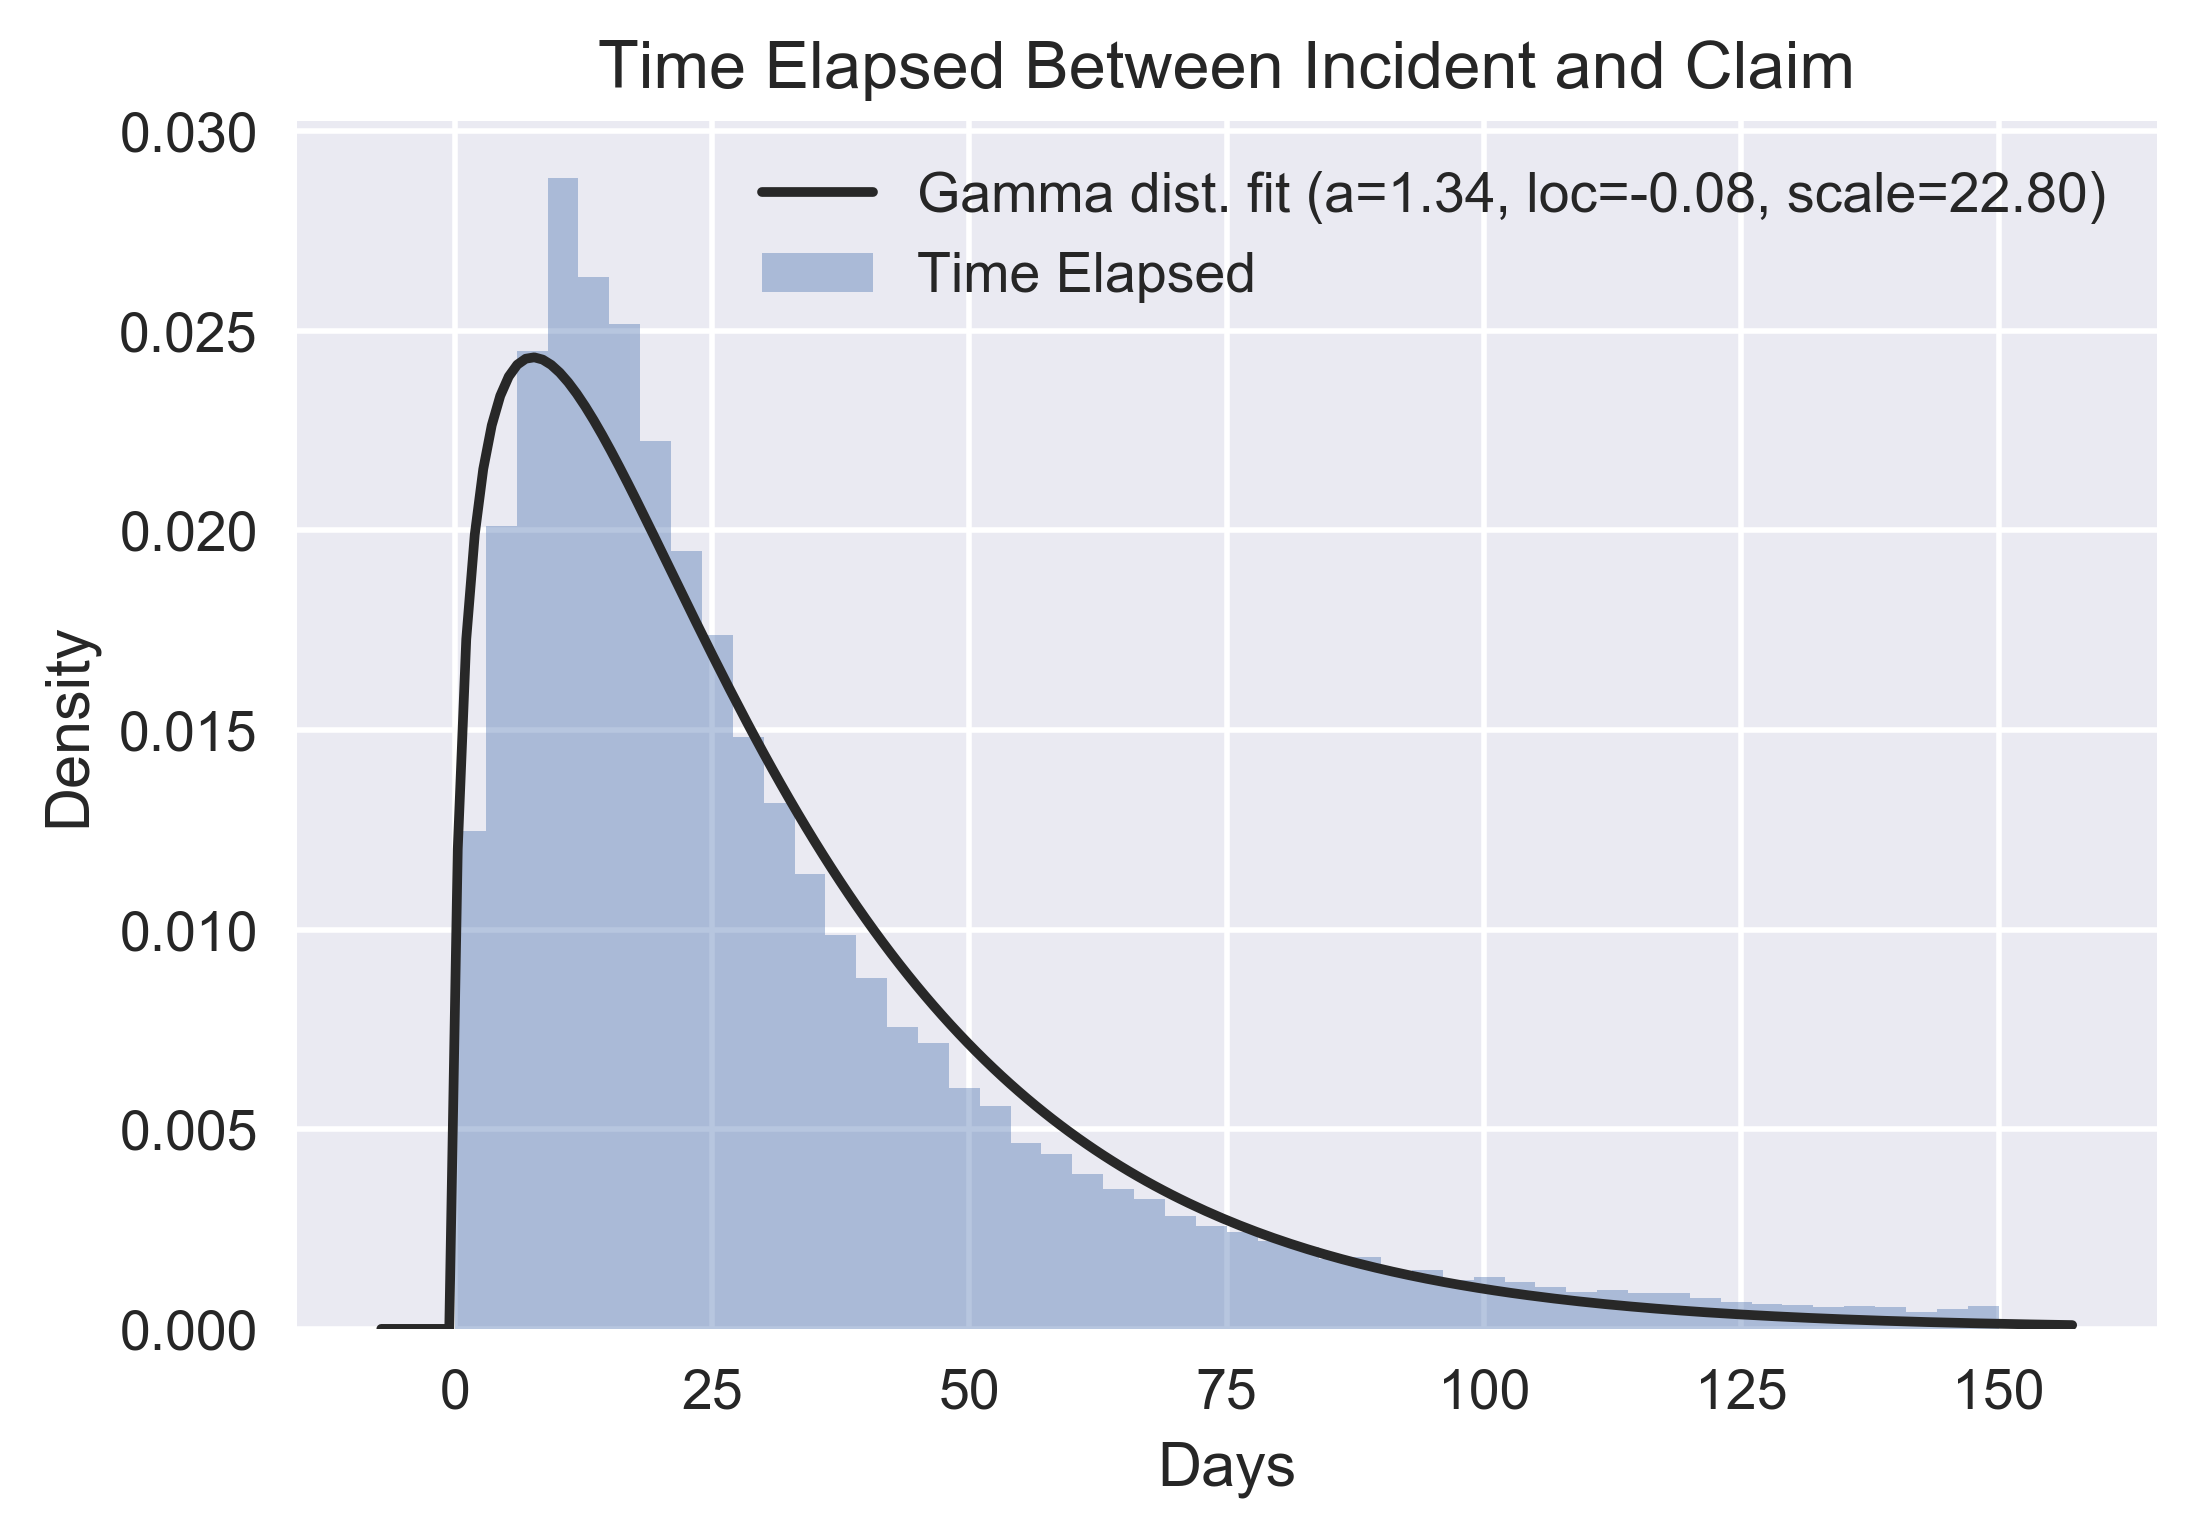
\includegraphics[keepaspectratio, width = 5cm]{../plots/wait_time}
	\hspace{1cm}
	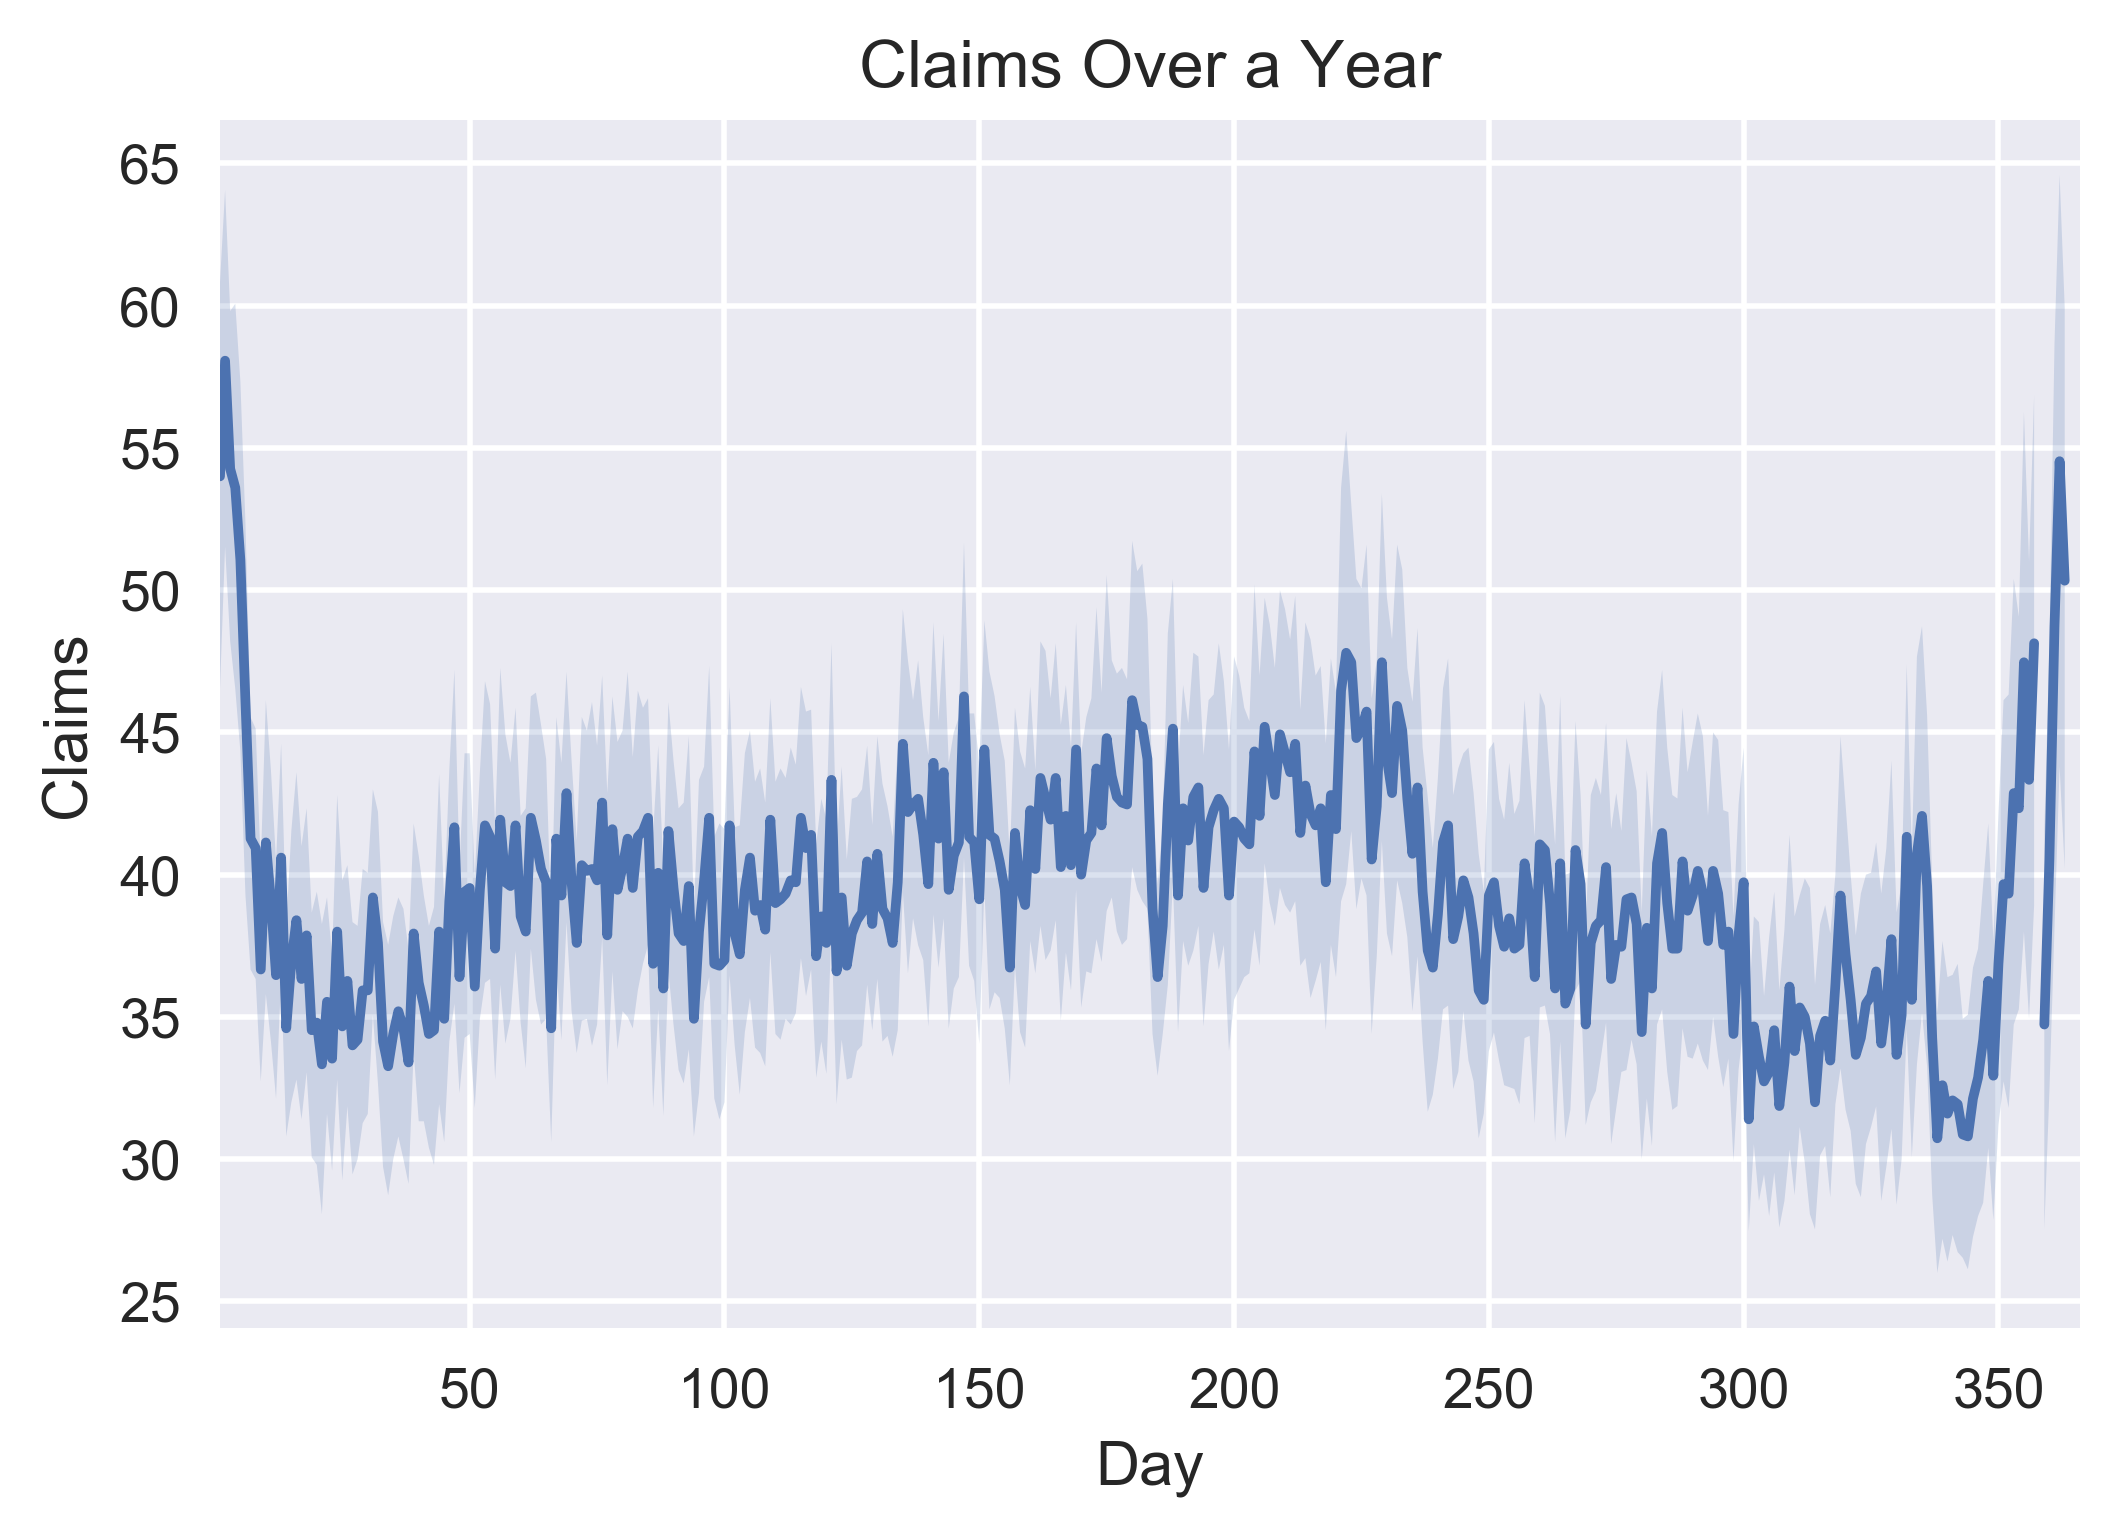
\includegraphics[keepaspectratio, width = 5cm]{../plots/avg_year_day}
\end{frame}

\begin{frame}
	\frametitle{Overview of the data set:}
	\begin{itemize}
		\item TSA claims data from 2002-2017  in~.pdf and~.xlsx format from \textcolor{blue}{\ul{https://www.dhs.gov/tsa-claims-data}}.

		\item Tables contain over 220,828 unique claims

		\item The 13 columns are:
			\begin{tabular}{c c c c}
				Claim Number & Date Received & Incident Date & Airport Code\\
				Airport Name & Airline Name & Claim Type & Claim Site\\
				Item Category & Claim Amount & Status & Close Amount\\
				Disposition
			\end{tabular}
	\end{itemize}
\end{frame}

\begin{frame}
	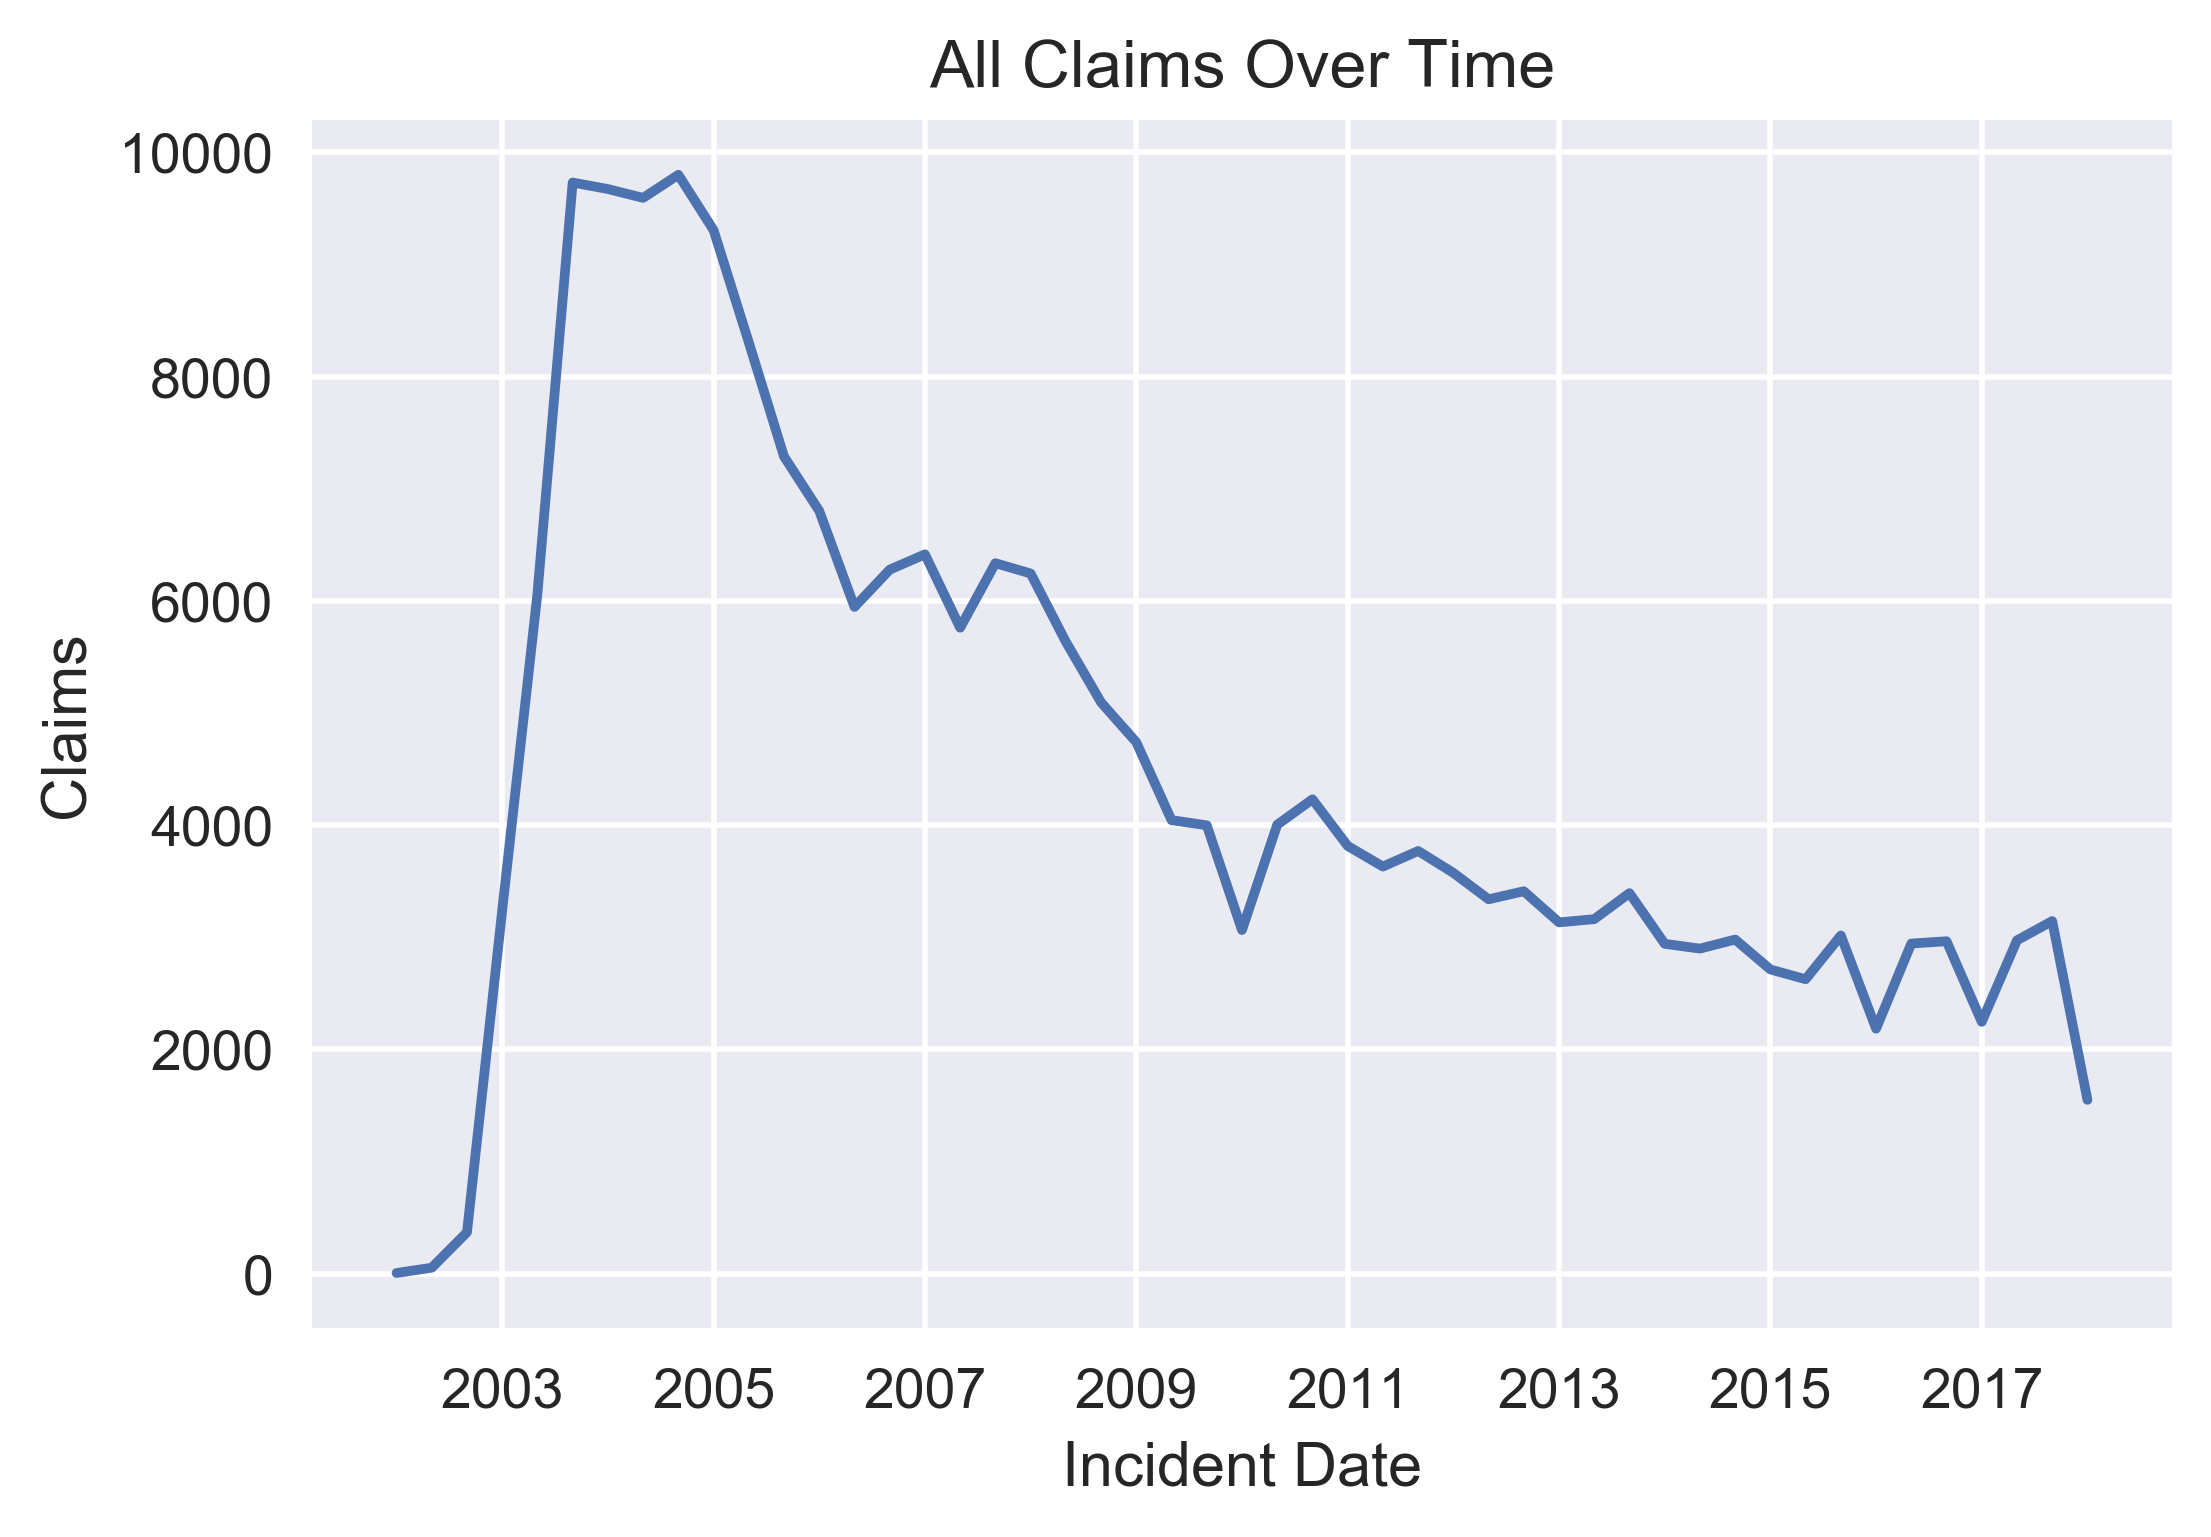
\includegraphics[keepaspectratio, width = \textwidth, height = \textheight]{../plots/all_claims}
\end{frame}

\begin{frame}
	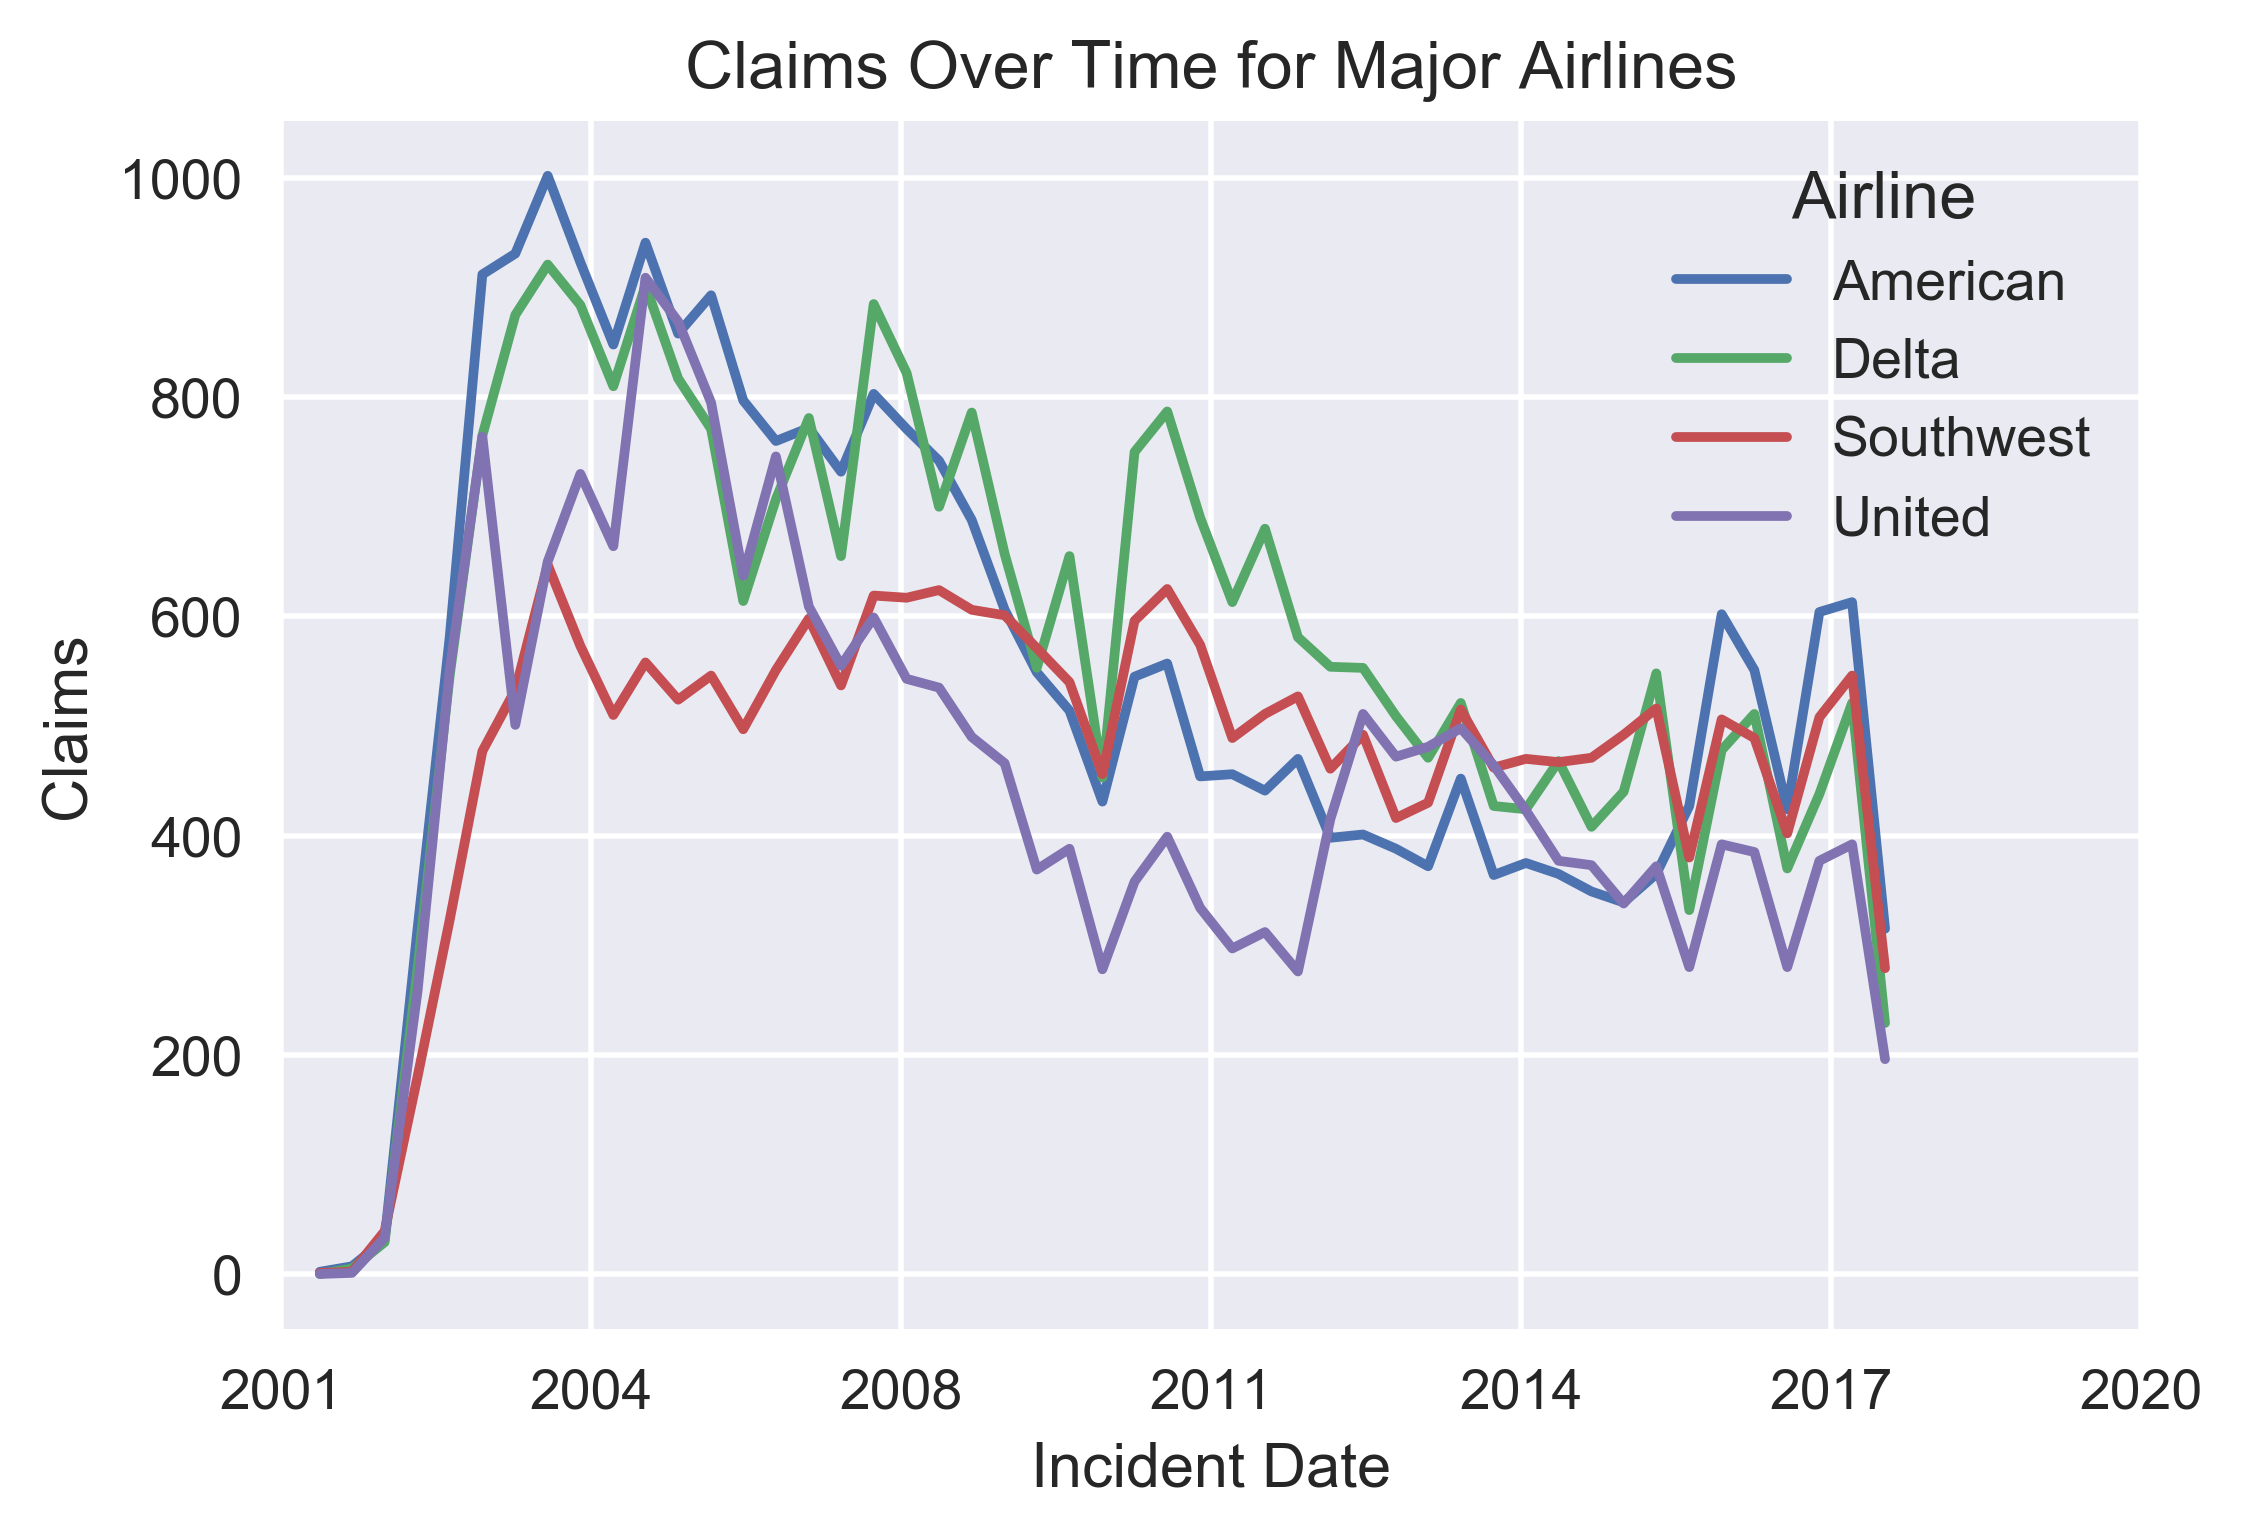
\includegraphics[keepaspectratio, width = \textwidth, height = \textheight]{../plots/by_airline}
\end{frame}

\begin{frame}
	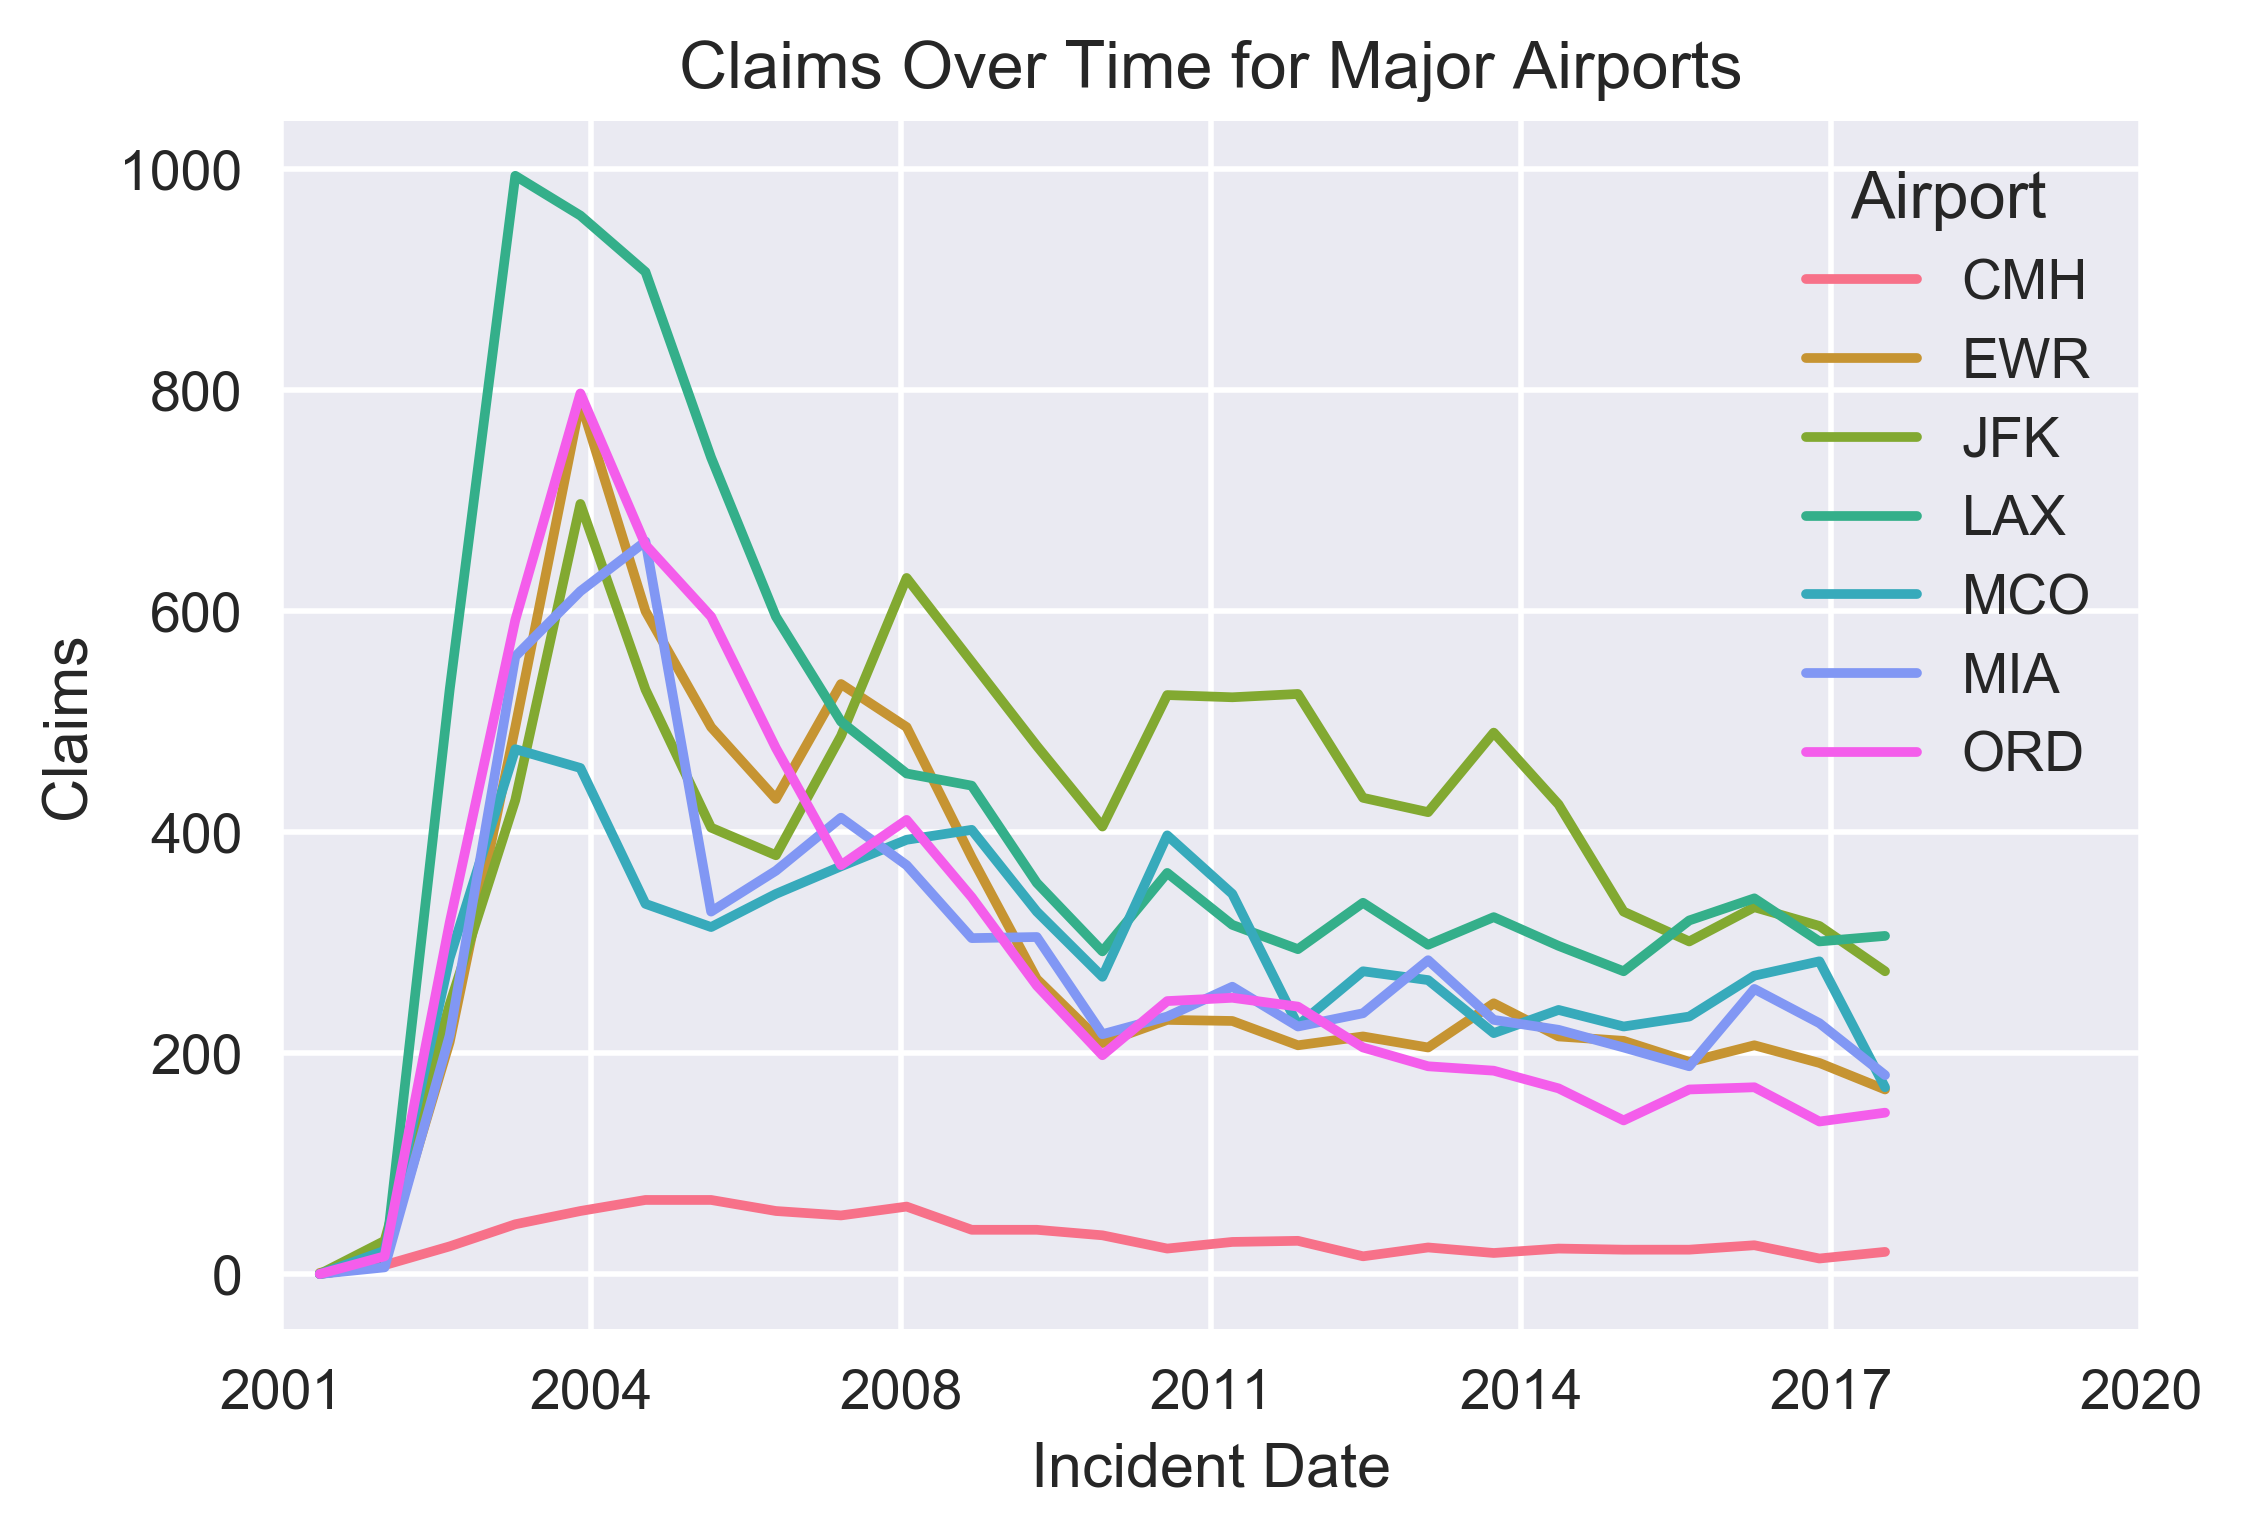
\includegraphics[keepaspectratio, width = \textwidth, height = \textheight]{../plots/by_airport}
\end{frame}

\begin{frame}
	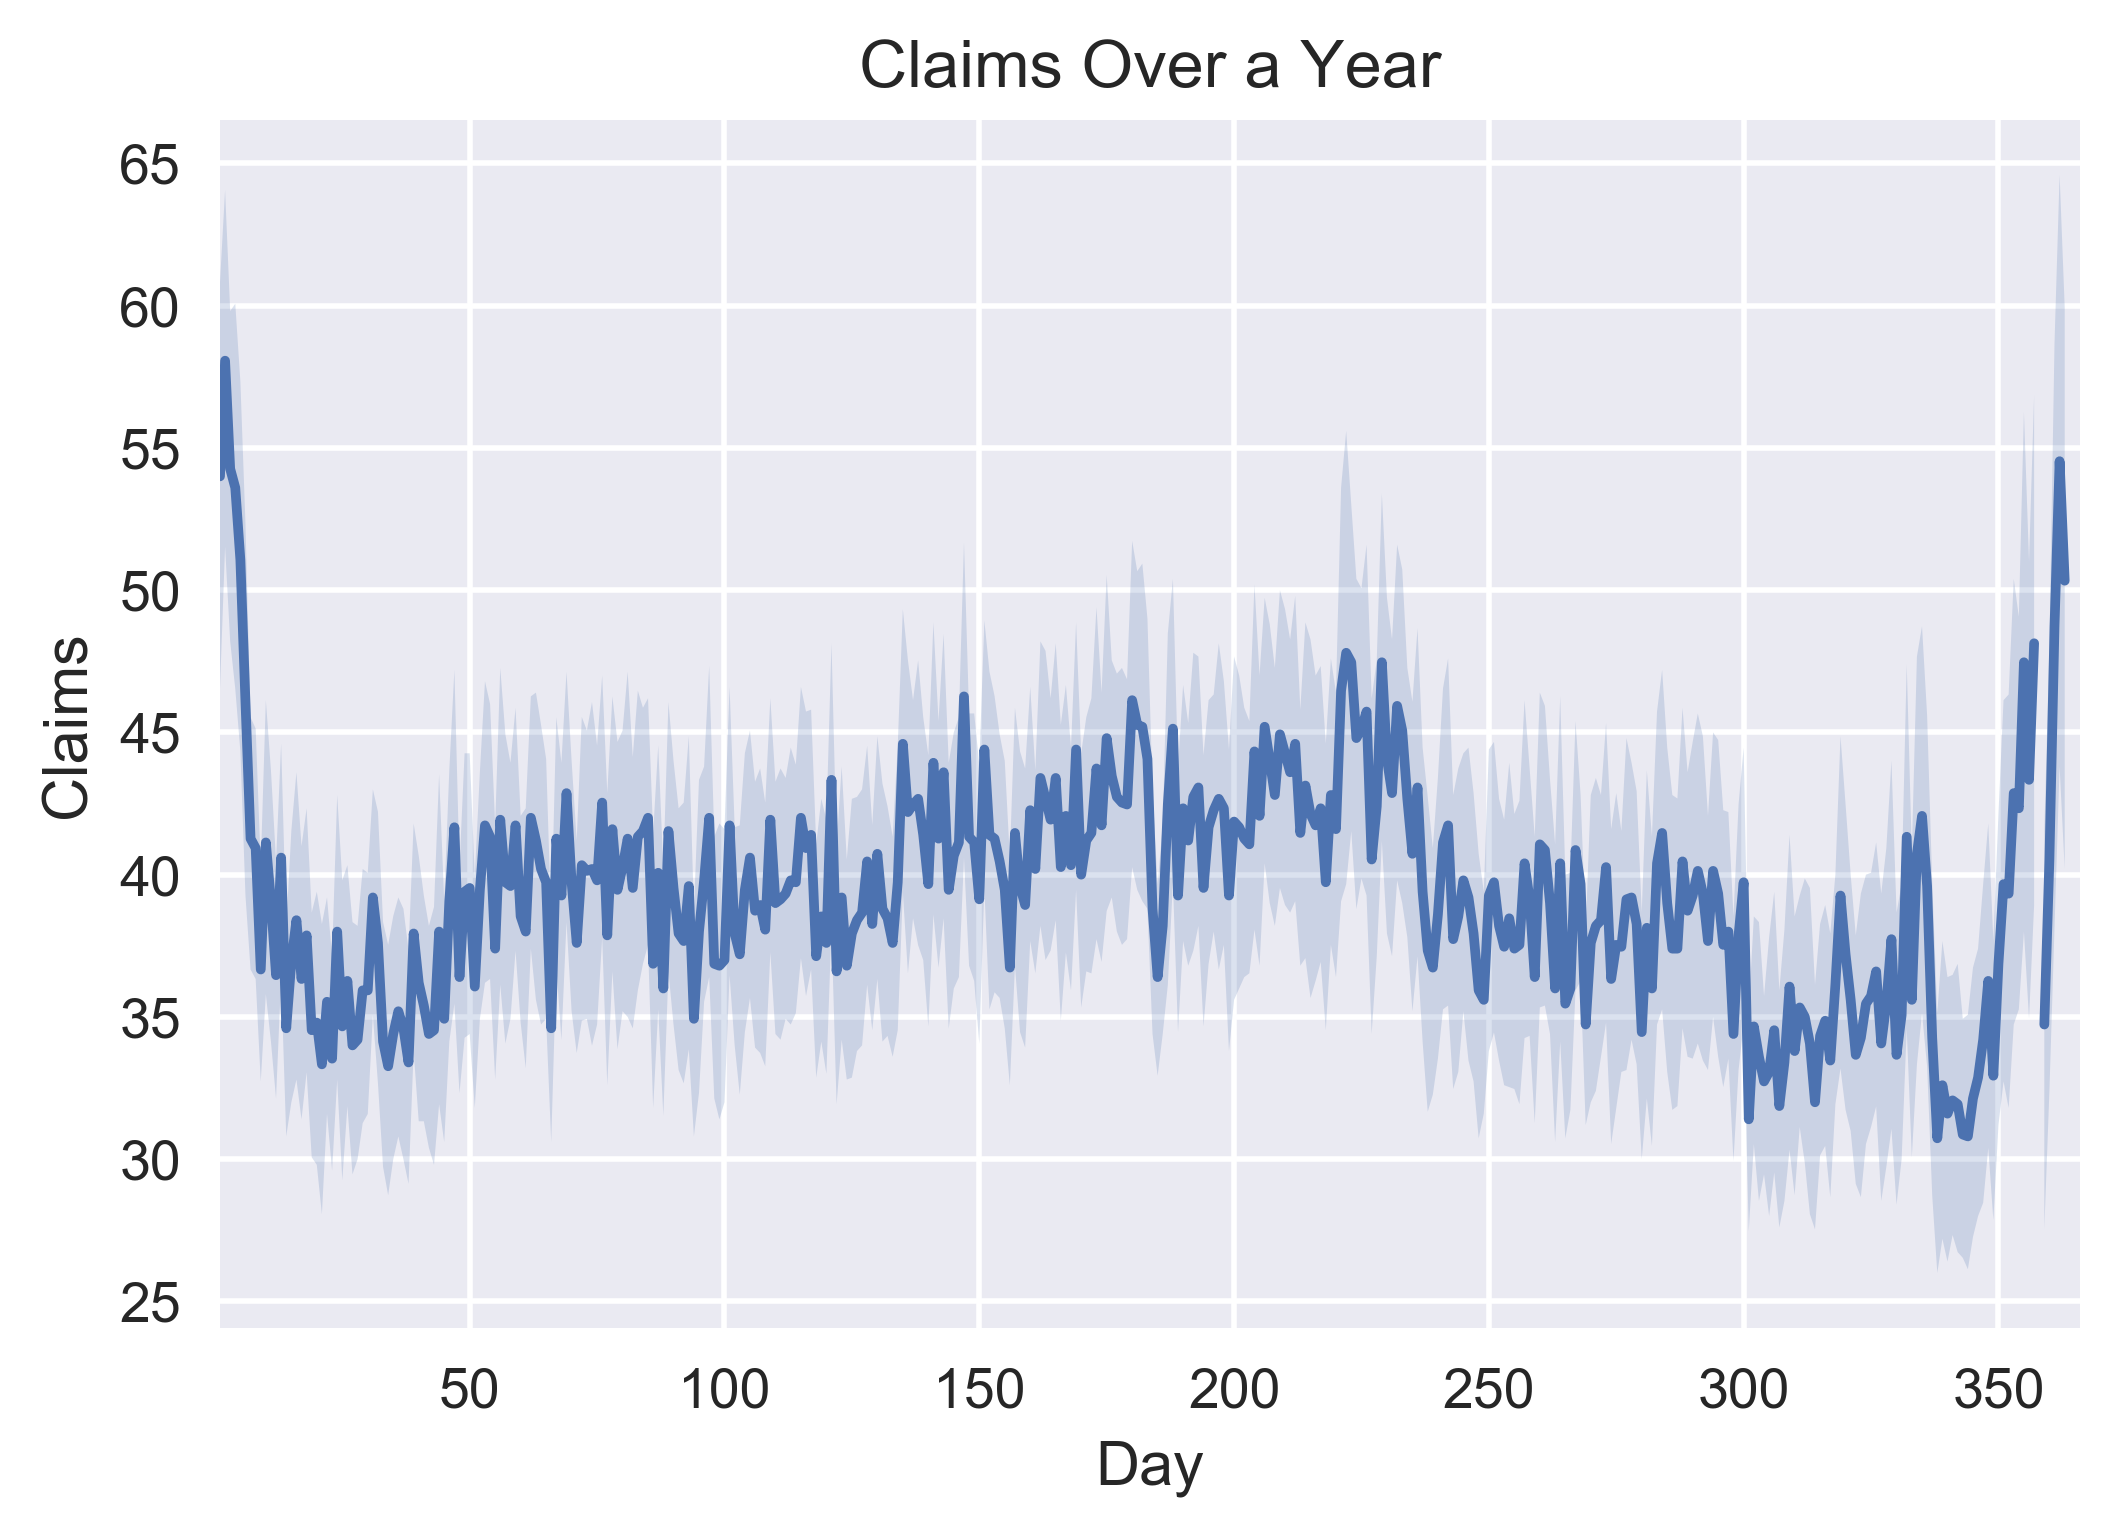
\includegraphics[keepaspectratio, width = \textwidth, height = \textheight]{../plots/avg_year_day}
\end{frame}

\begin{frame}
	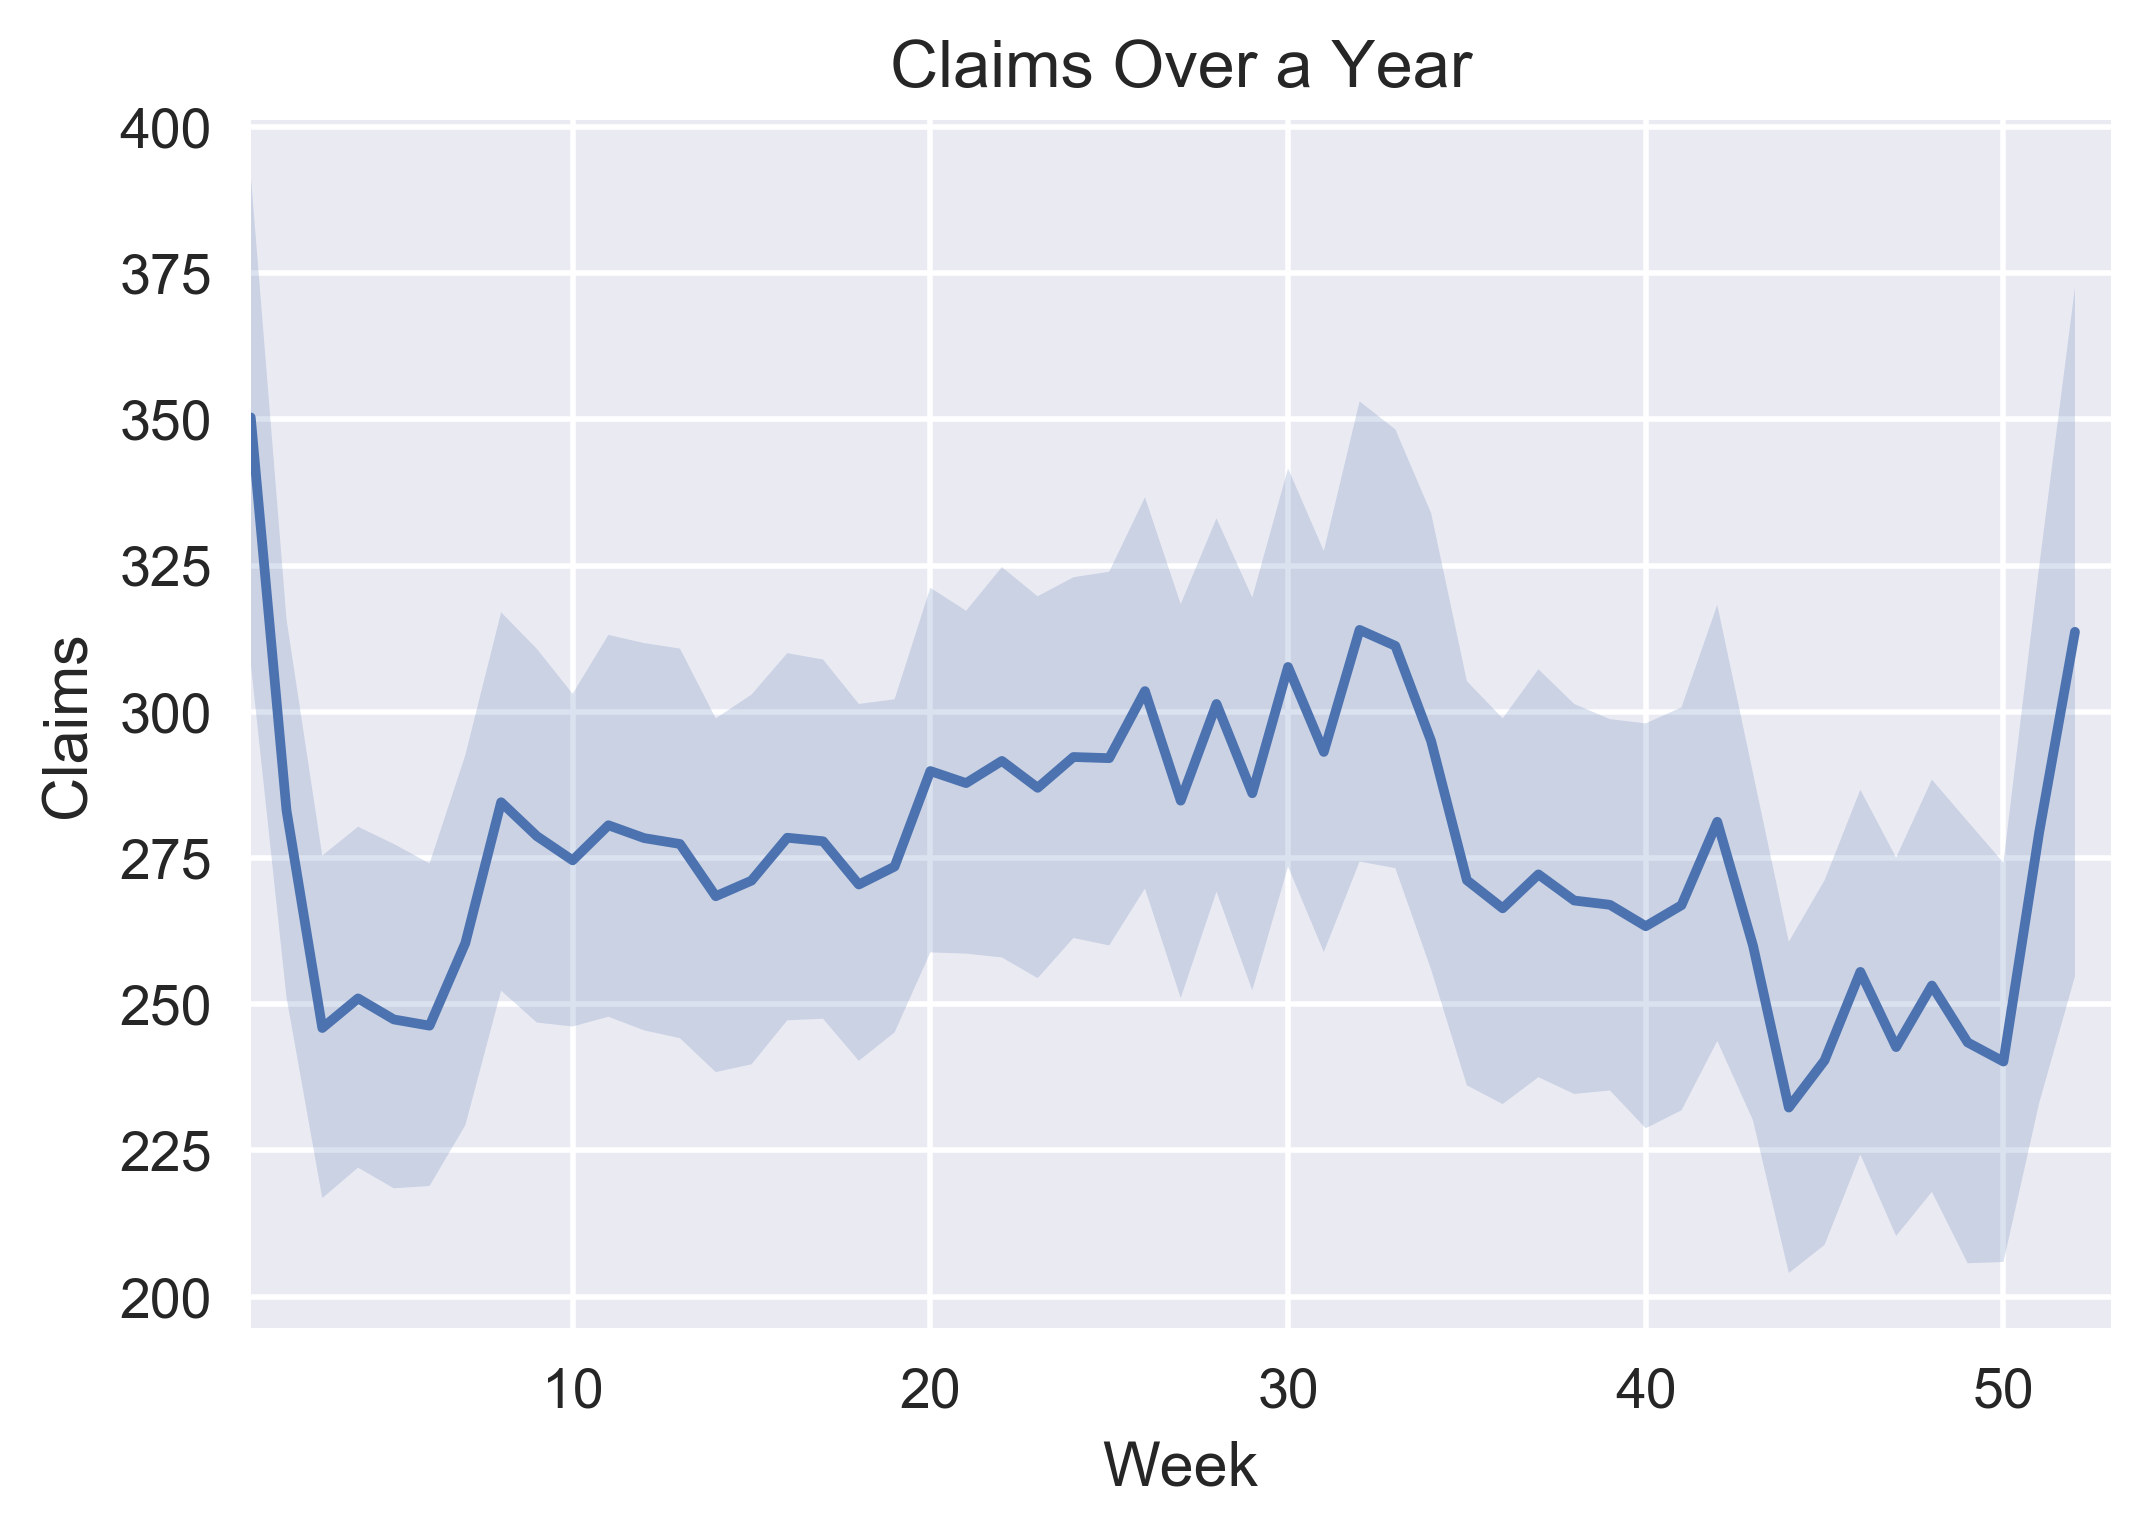
\includegraphics[keepaspectratio, width = \textwidth, height = \textheight]{../plots/avg_year}
\end{frame}

\begin{frame}
	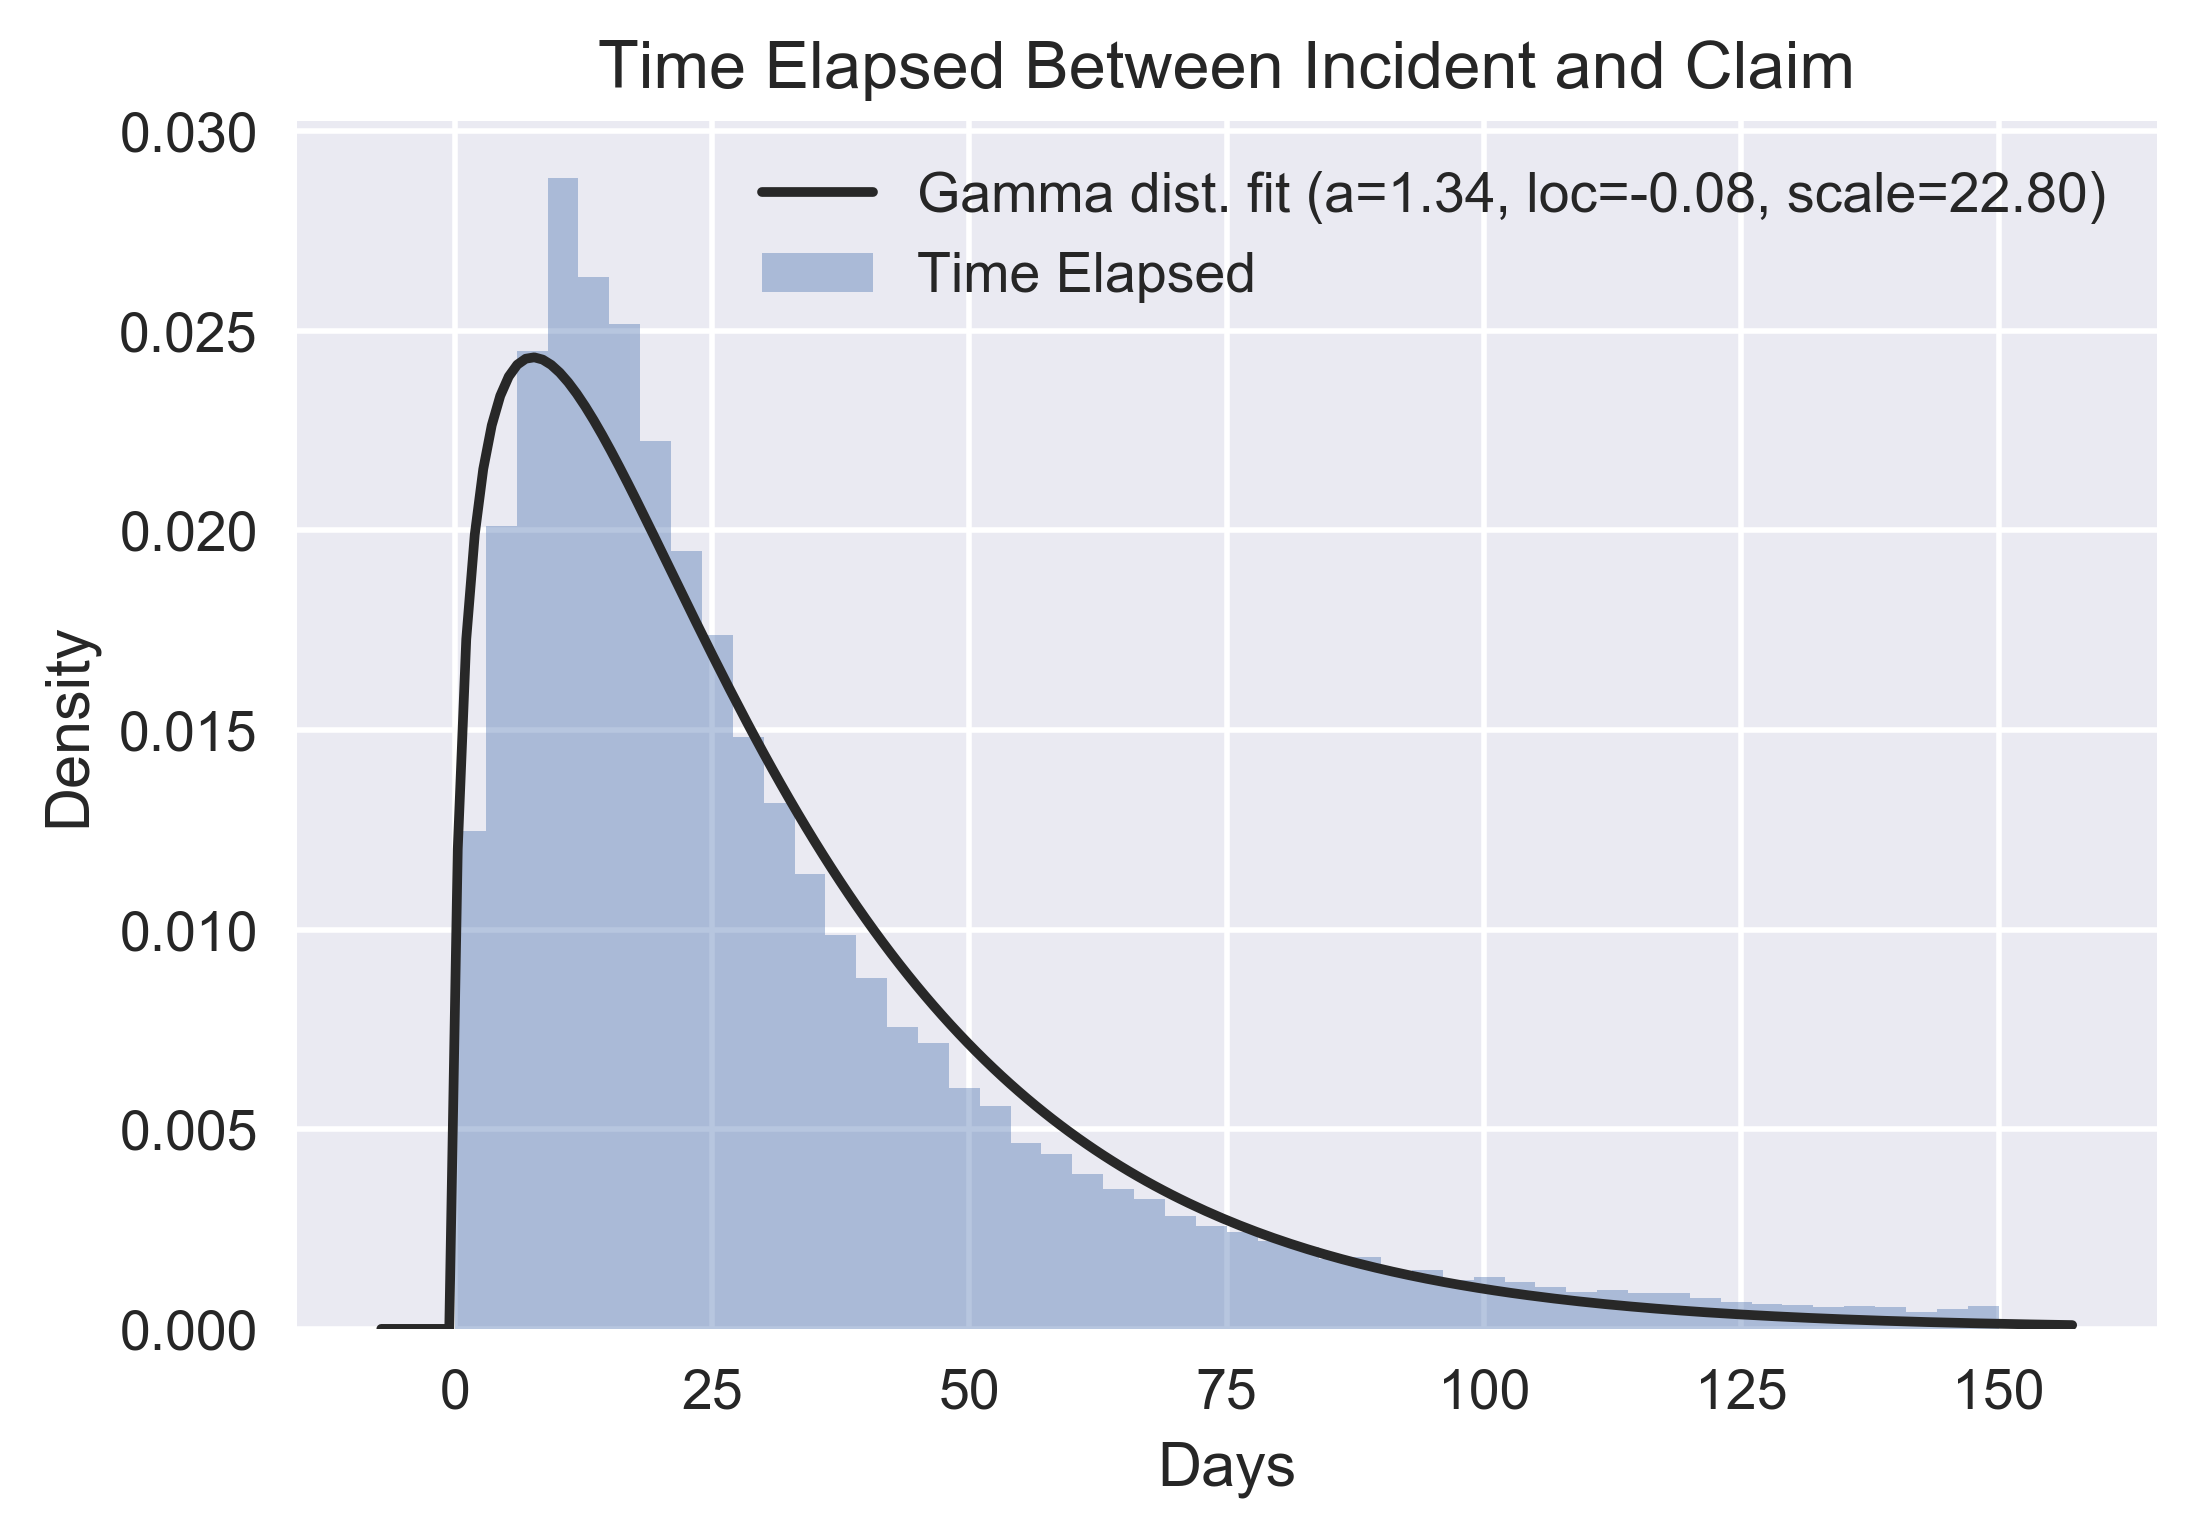
\includegraphics[keepaspectratio, width = \textwidth, height = \textheight]{../plots/wait_time}
\end{frame}

\begin{frame}
	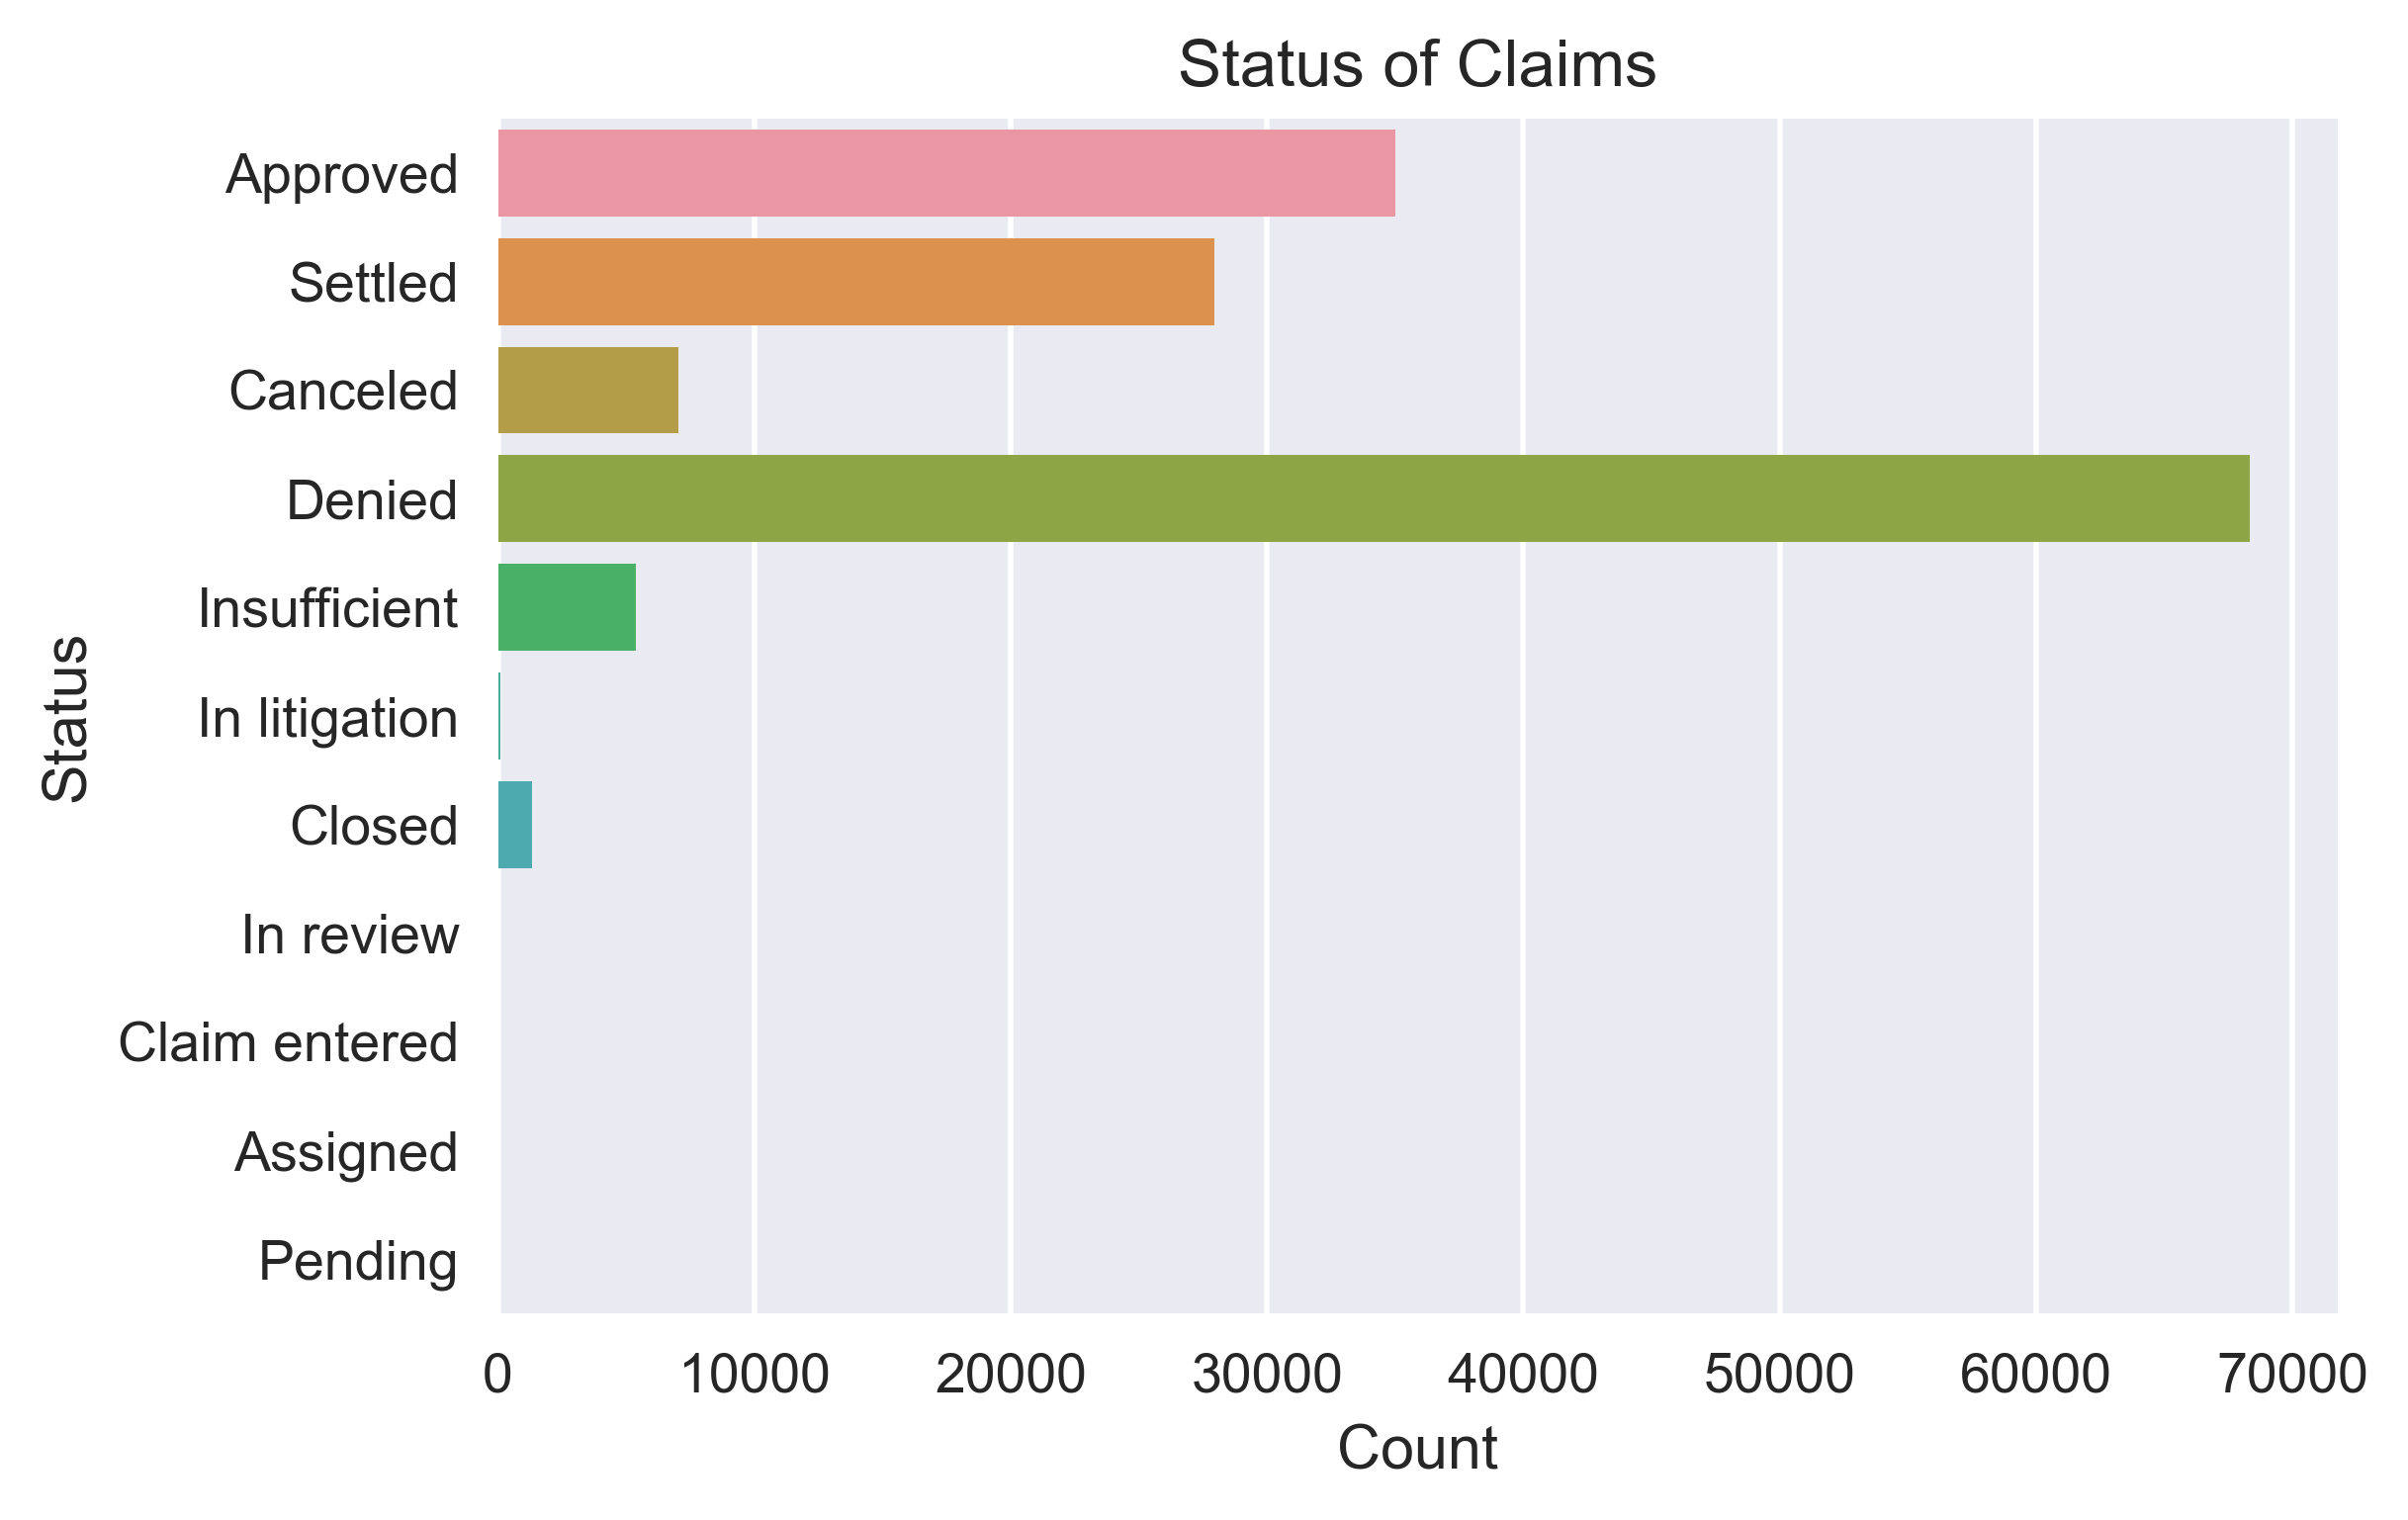
\includegraphics[keepaspectratio, width = \textwidth, height = \textheight]{../plots/status}
\end{frame}

\begin{frame}
	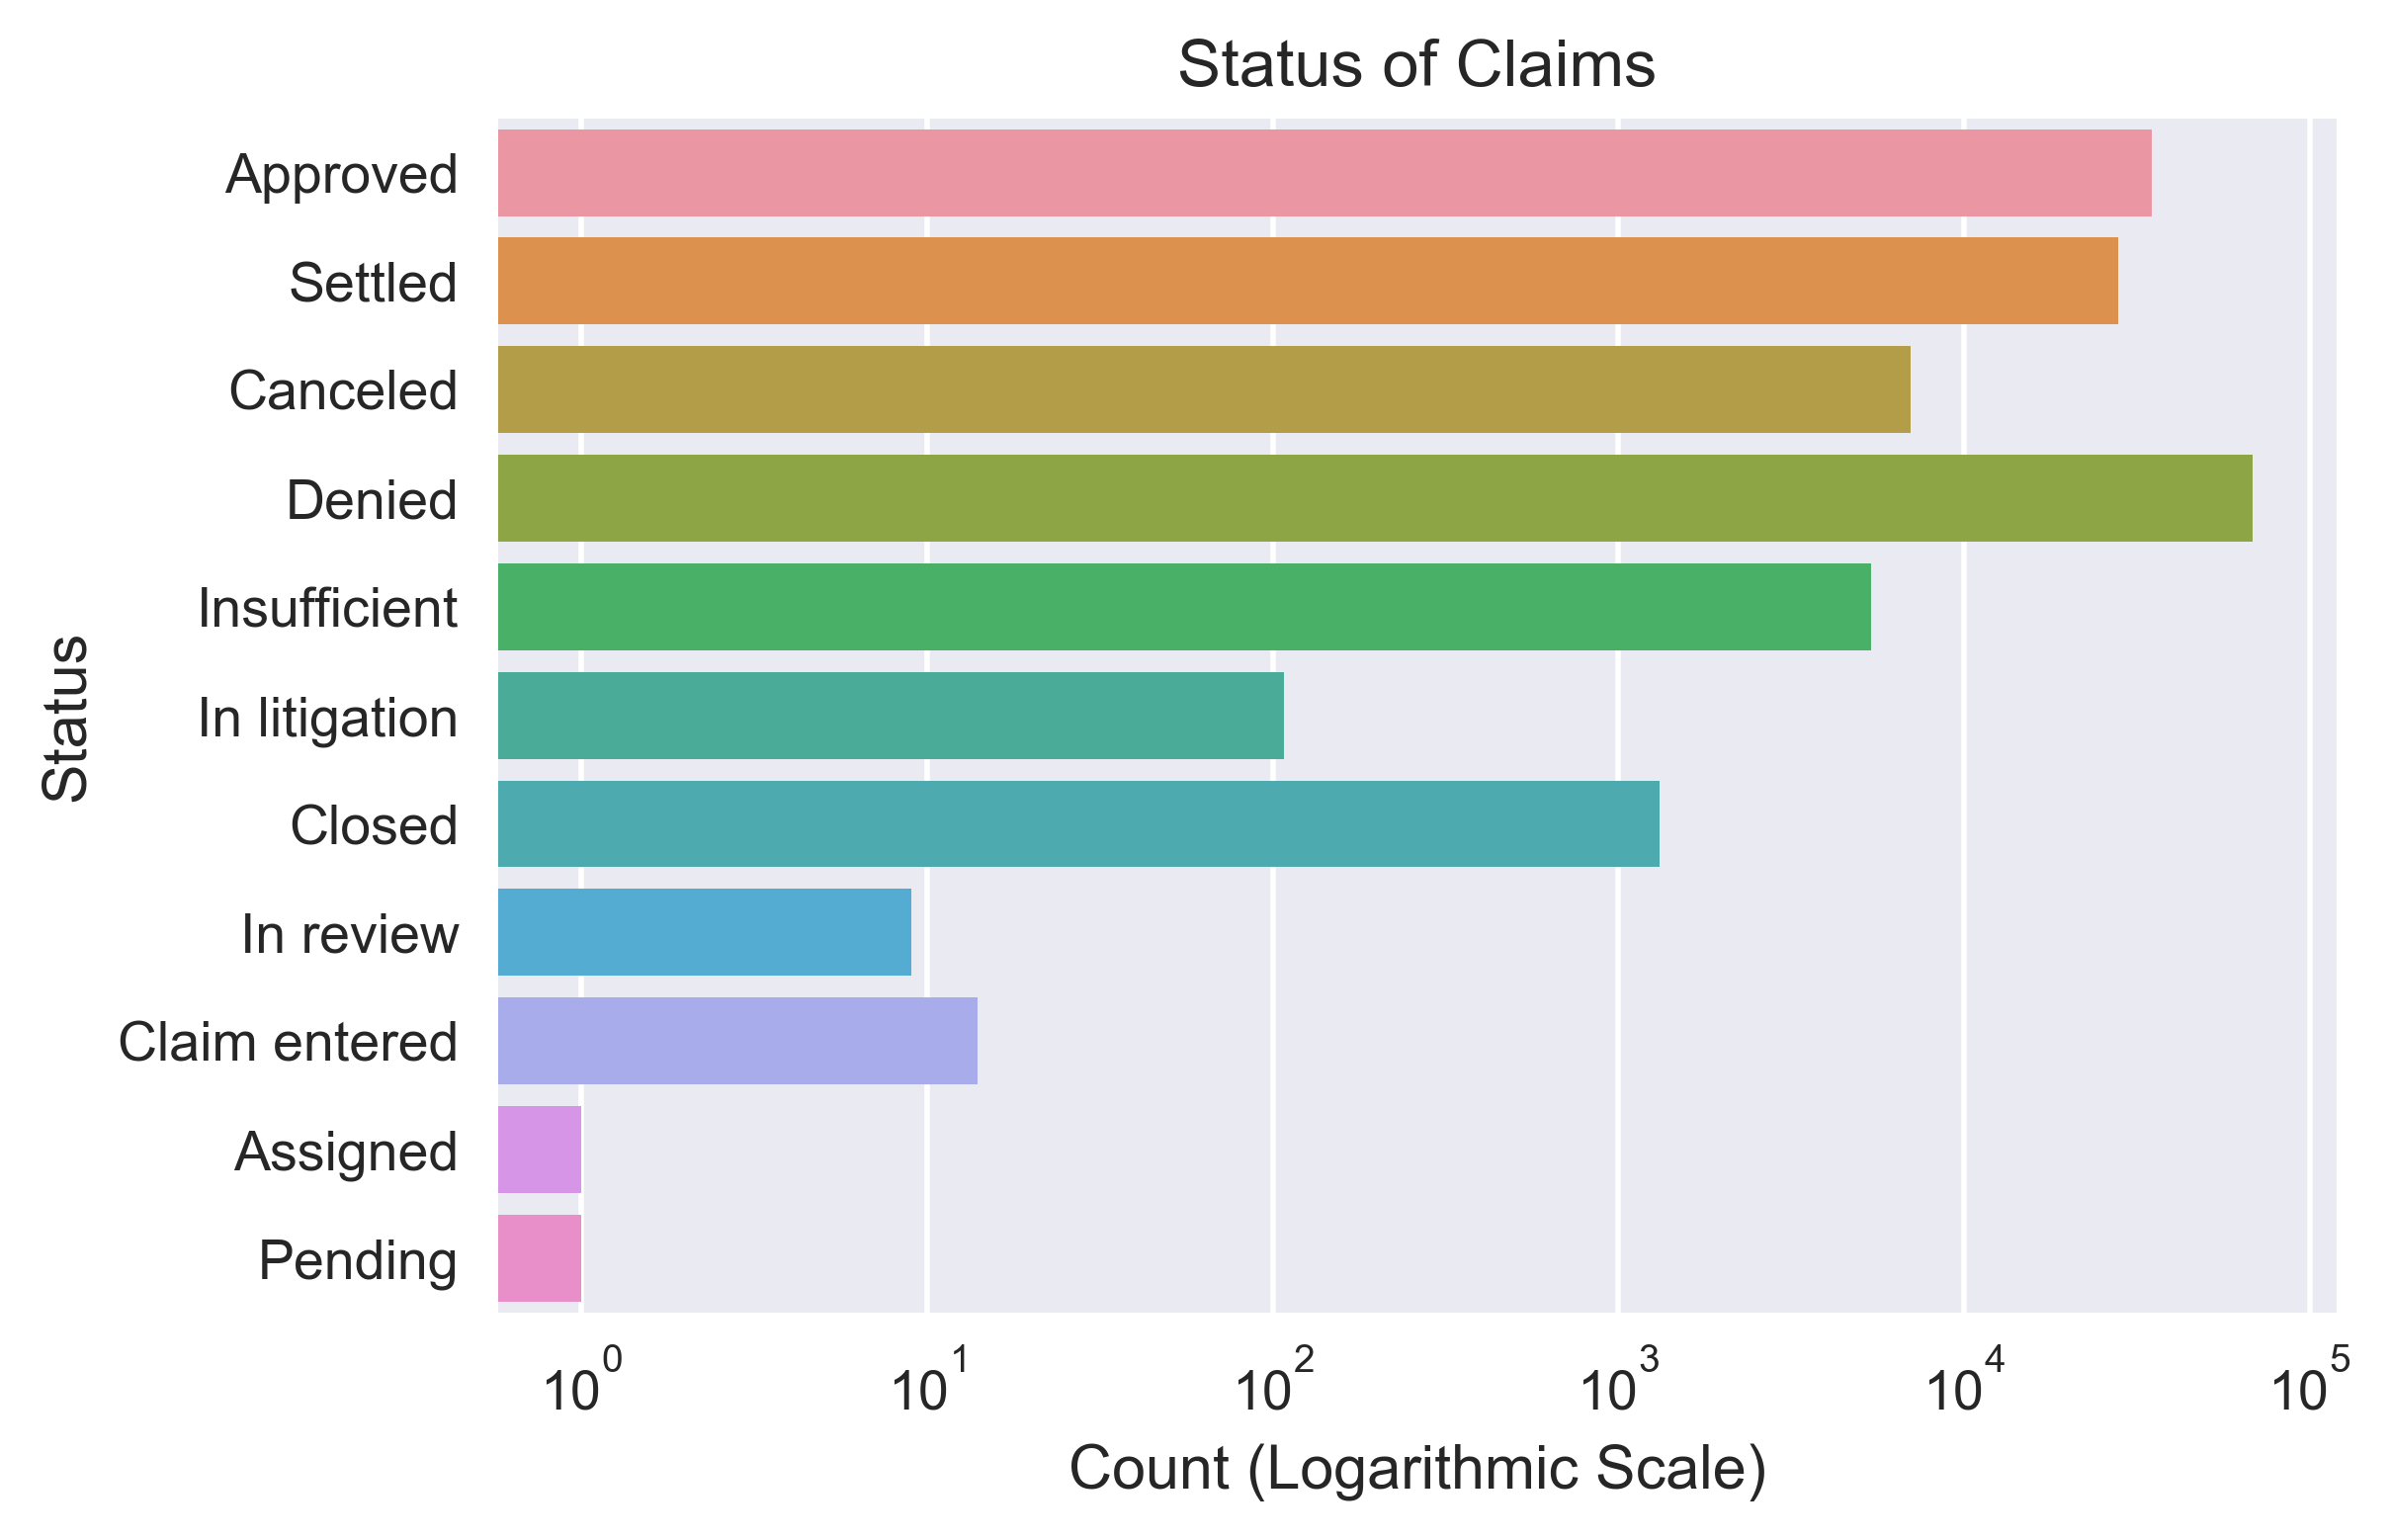
\includegraphics[keepaspectratio, width = \textwidth, height = \textheight]{../plots/log_status}
\end{frame}

\begin{frame}
	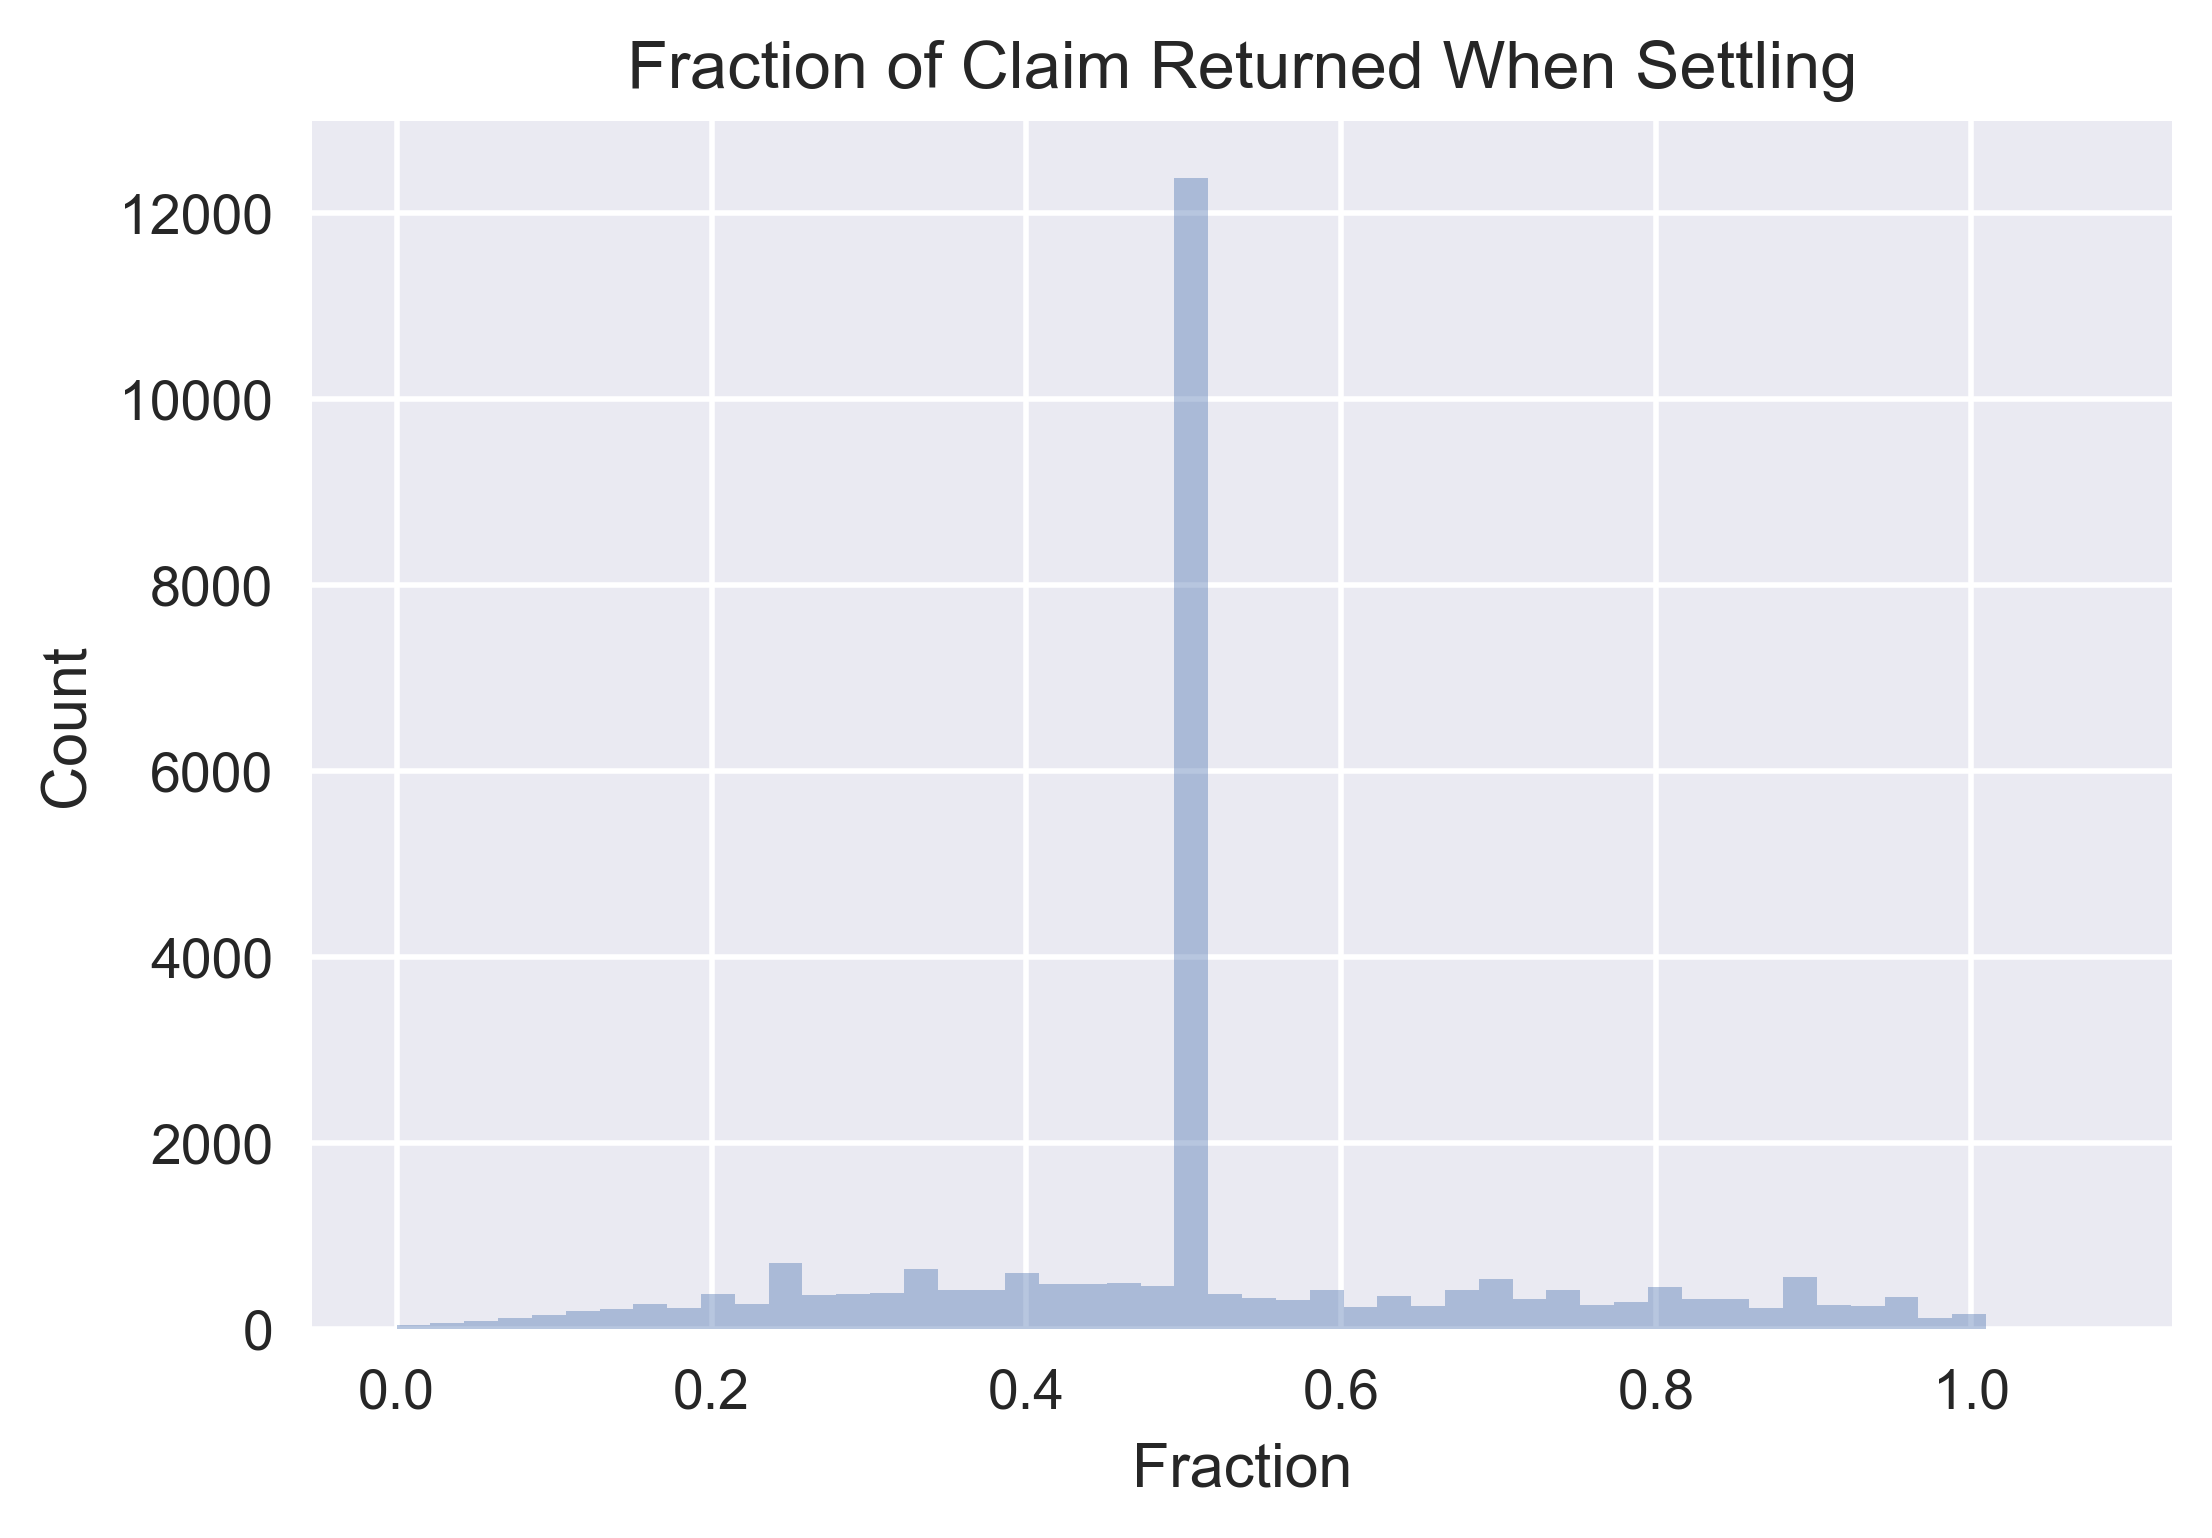
\includegraphics[keepaspectratio, width = \textwidth, height = \textheight]{../plots/settled}
\end{frame}

\begin{frame}
	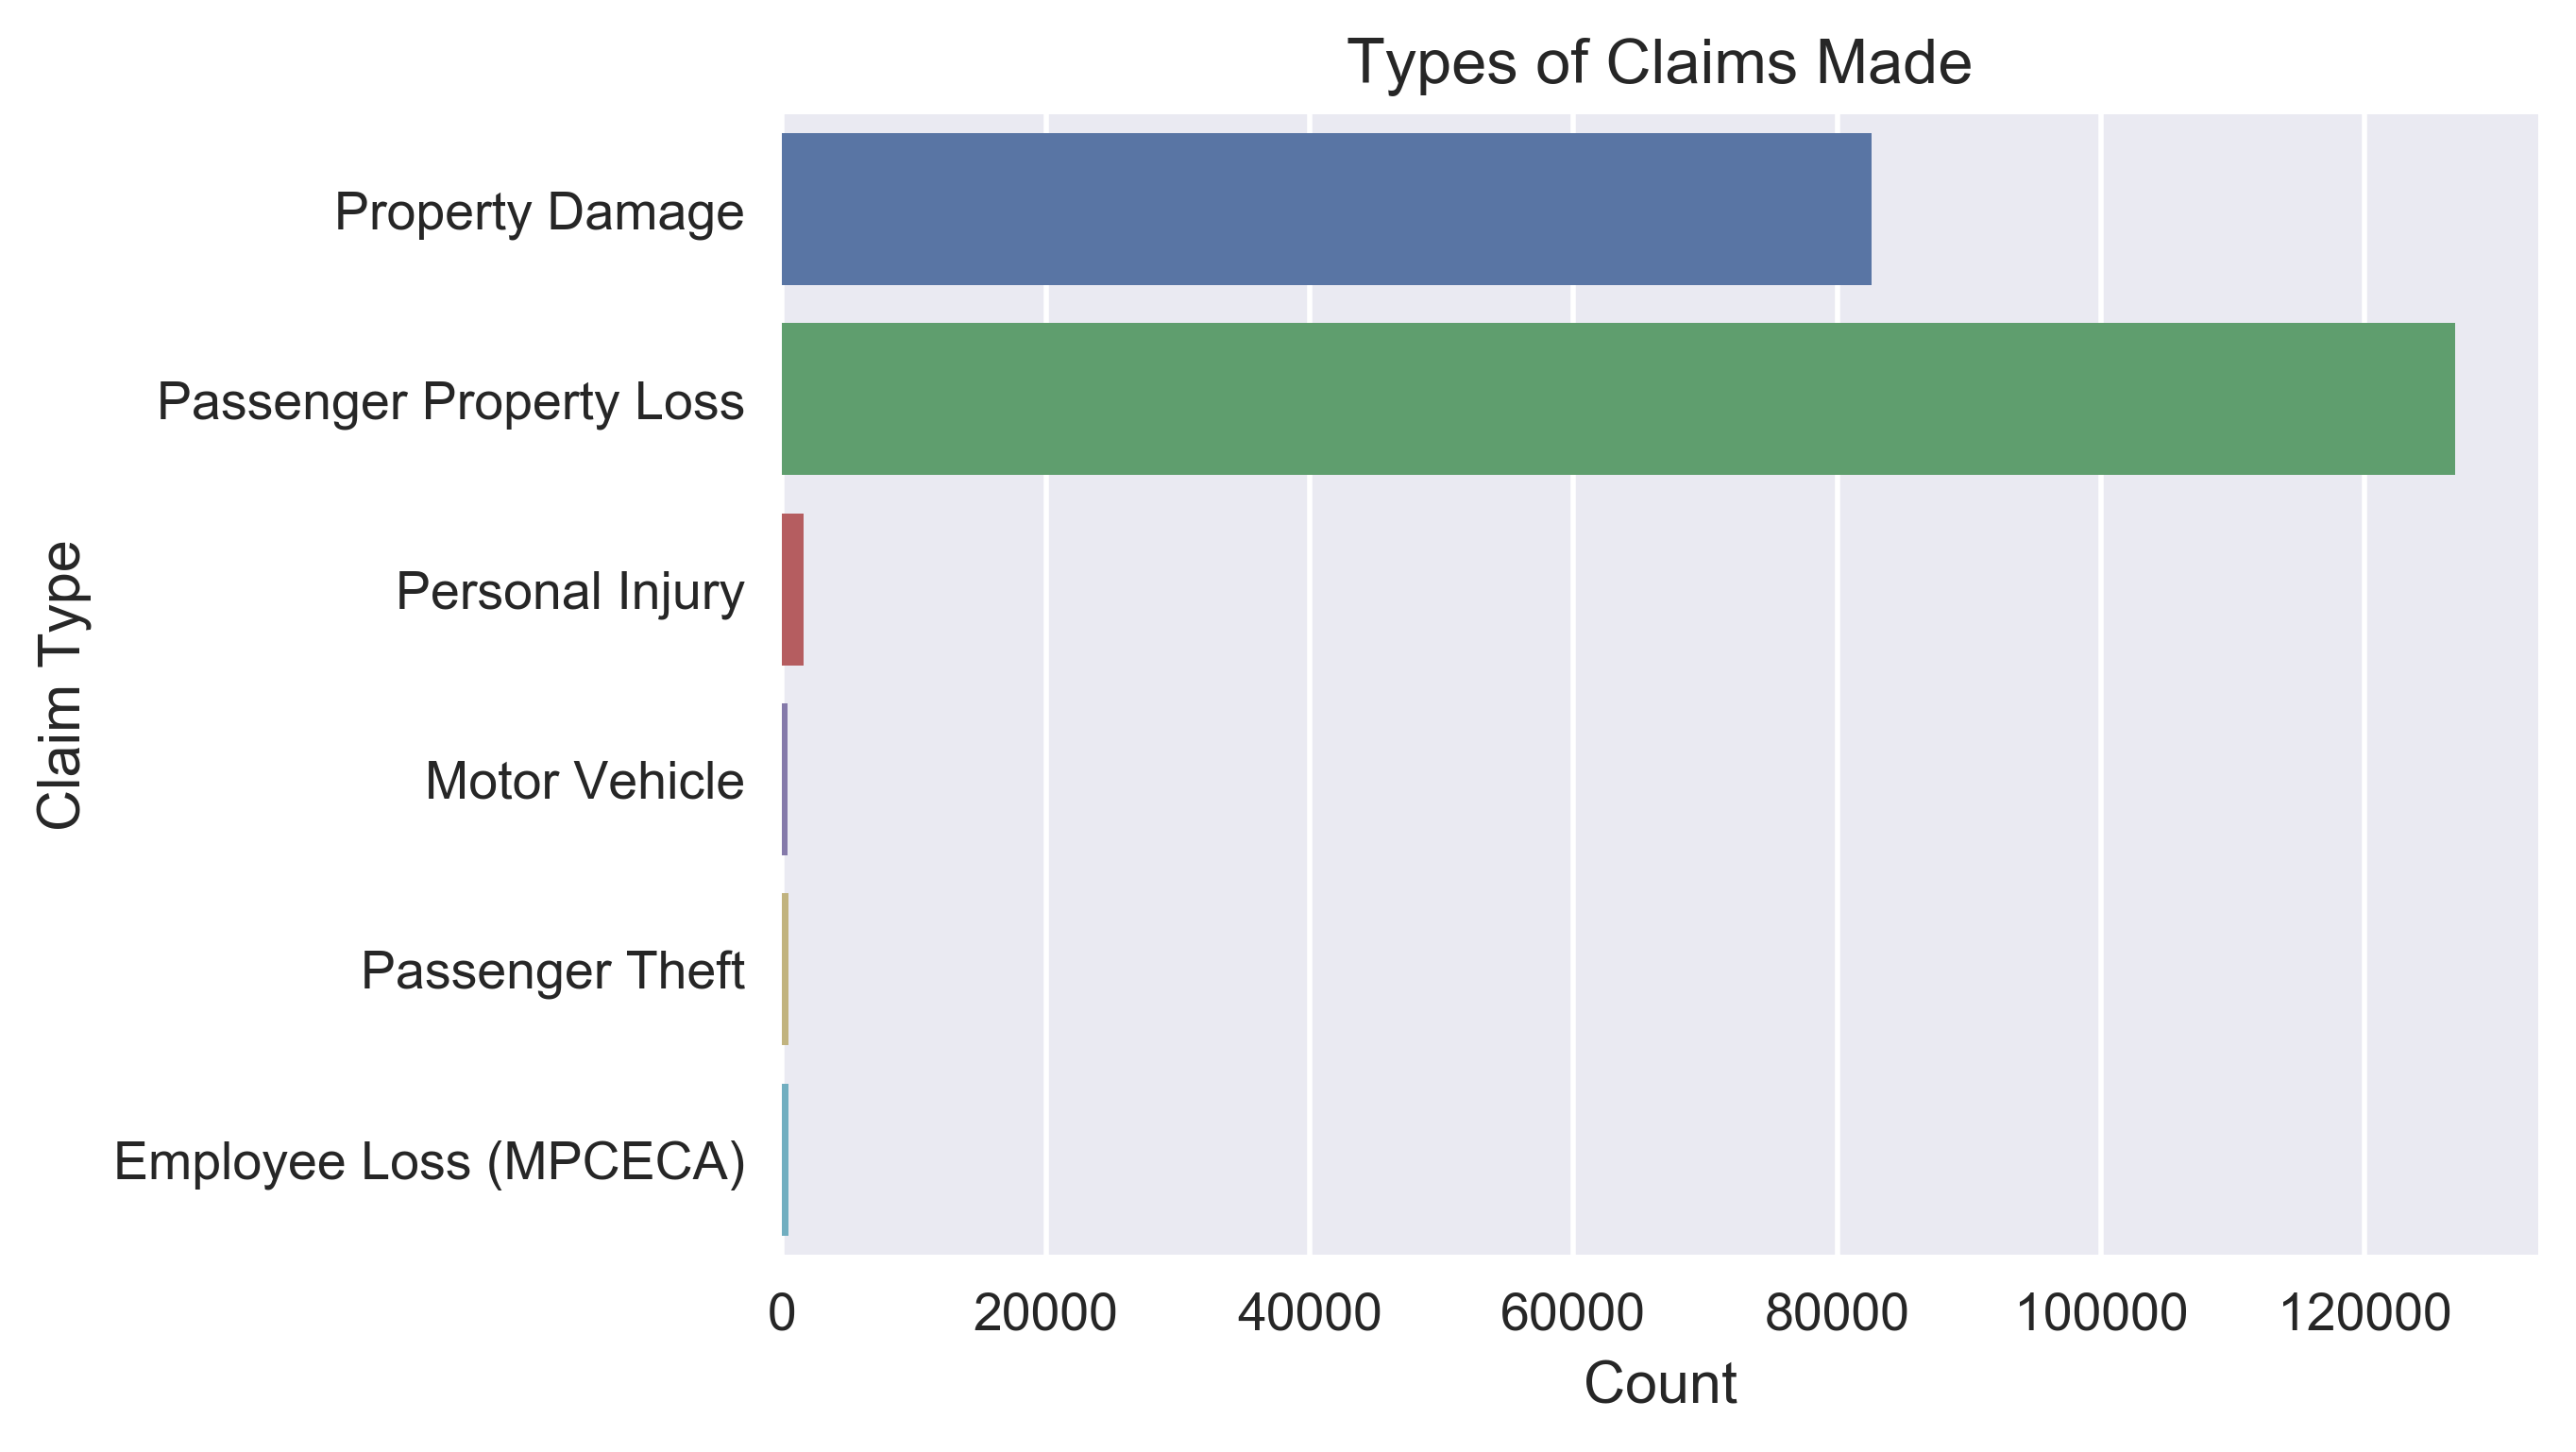
\includegraphics[keepaspectratio, width = \textwidth, height = \textheight]{../plots/type}
\end{frame}

\begin{frame}
	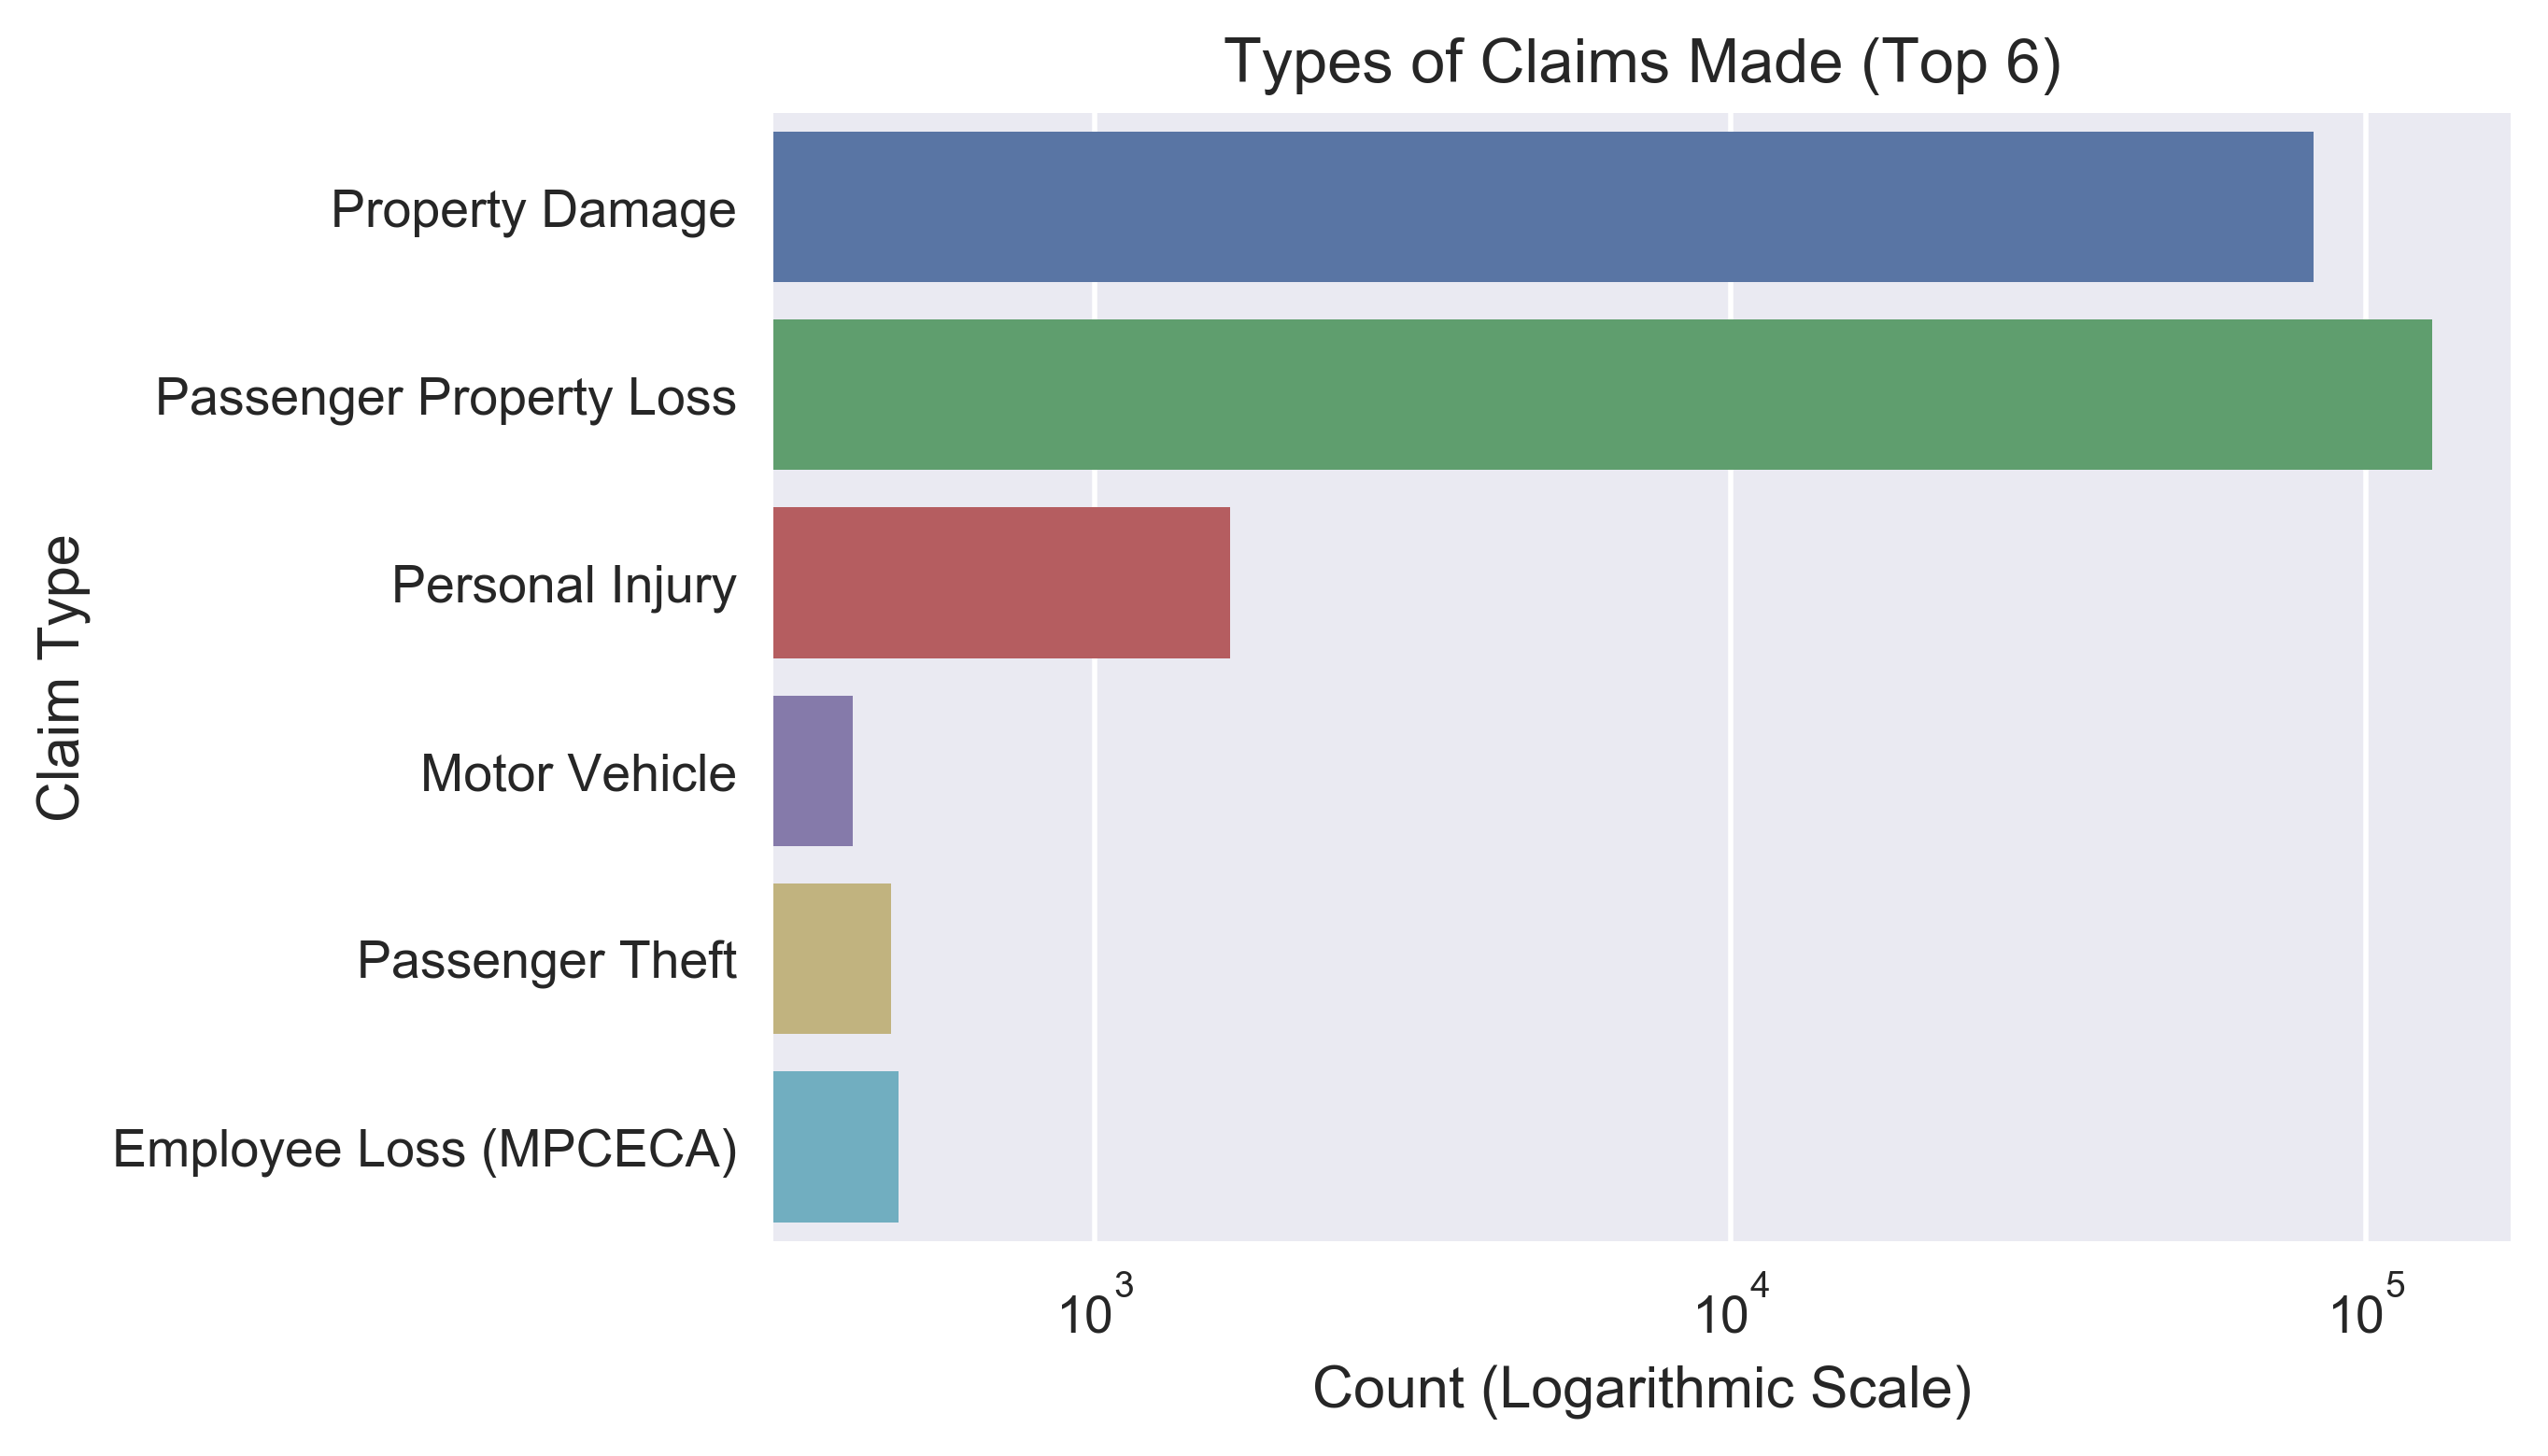
\includegraphics[keepaspectratio, width = \textwidth, height = \textheight]{../plots/log_type}
\end{frame}

\begin{frame}
	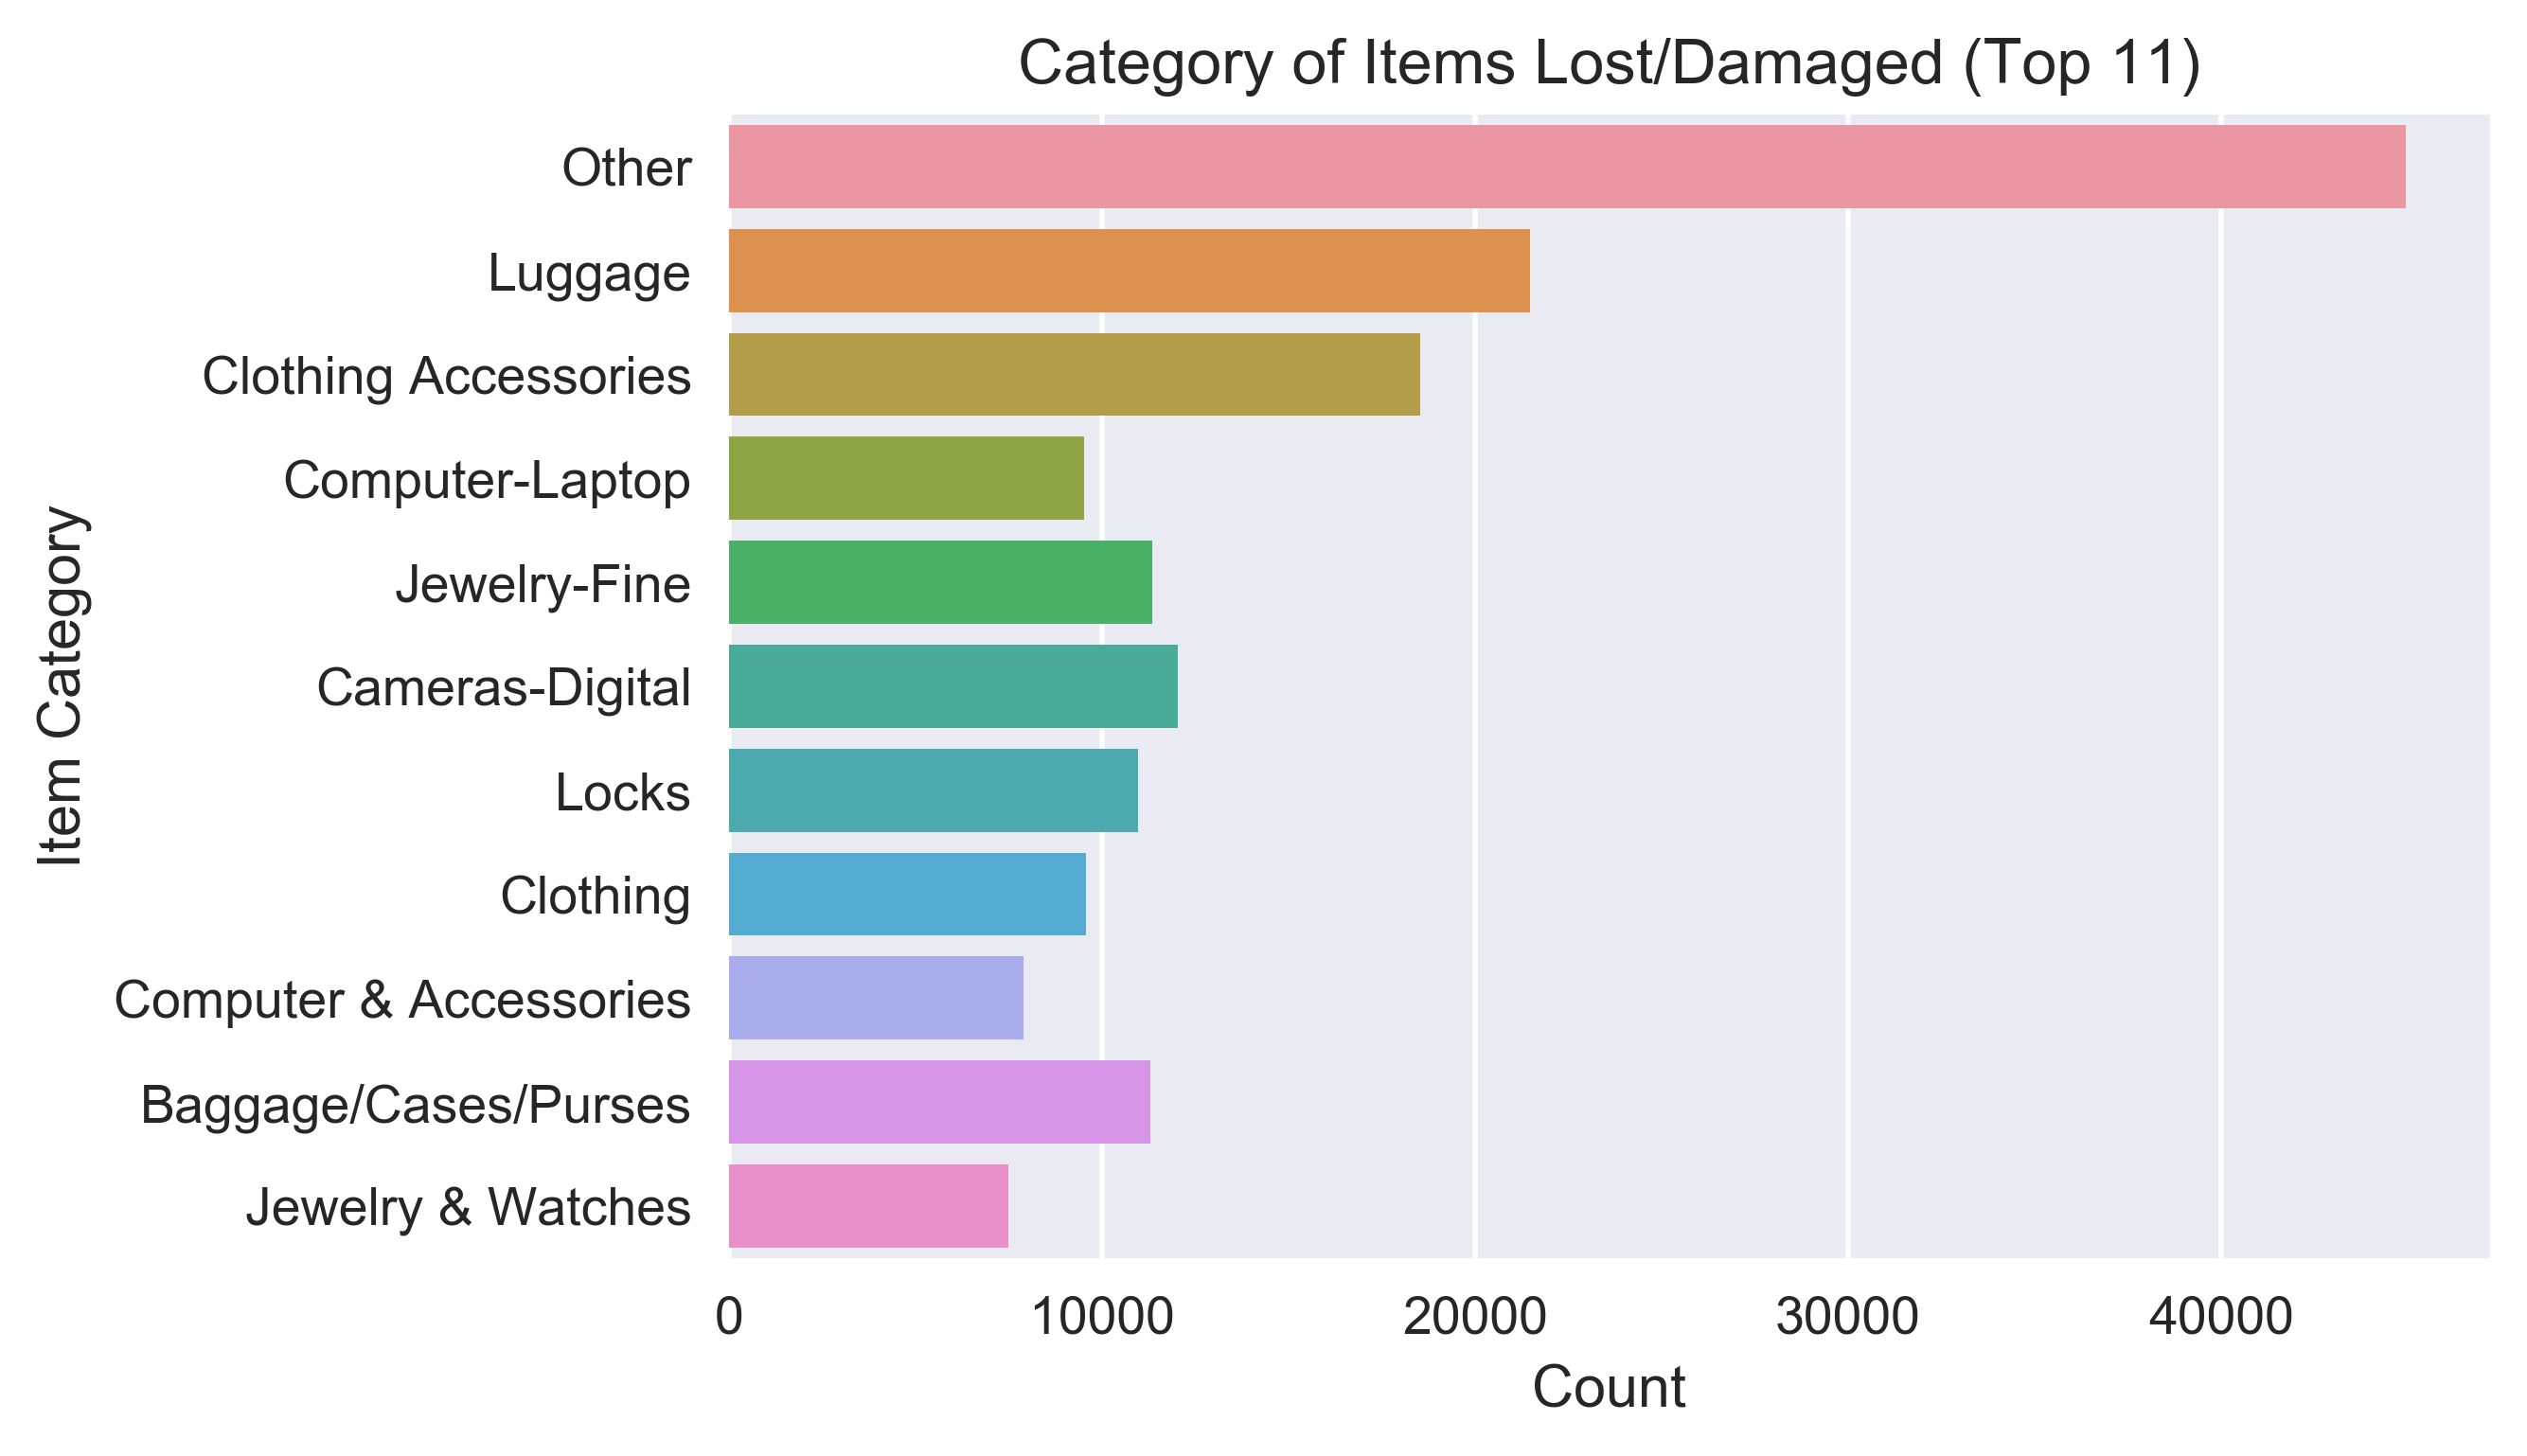
\includegraphics[keepaspectratio, width = \textwidth, height = \textheight]{../plots/items}
\end{frame}

\begin{frame}
	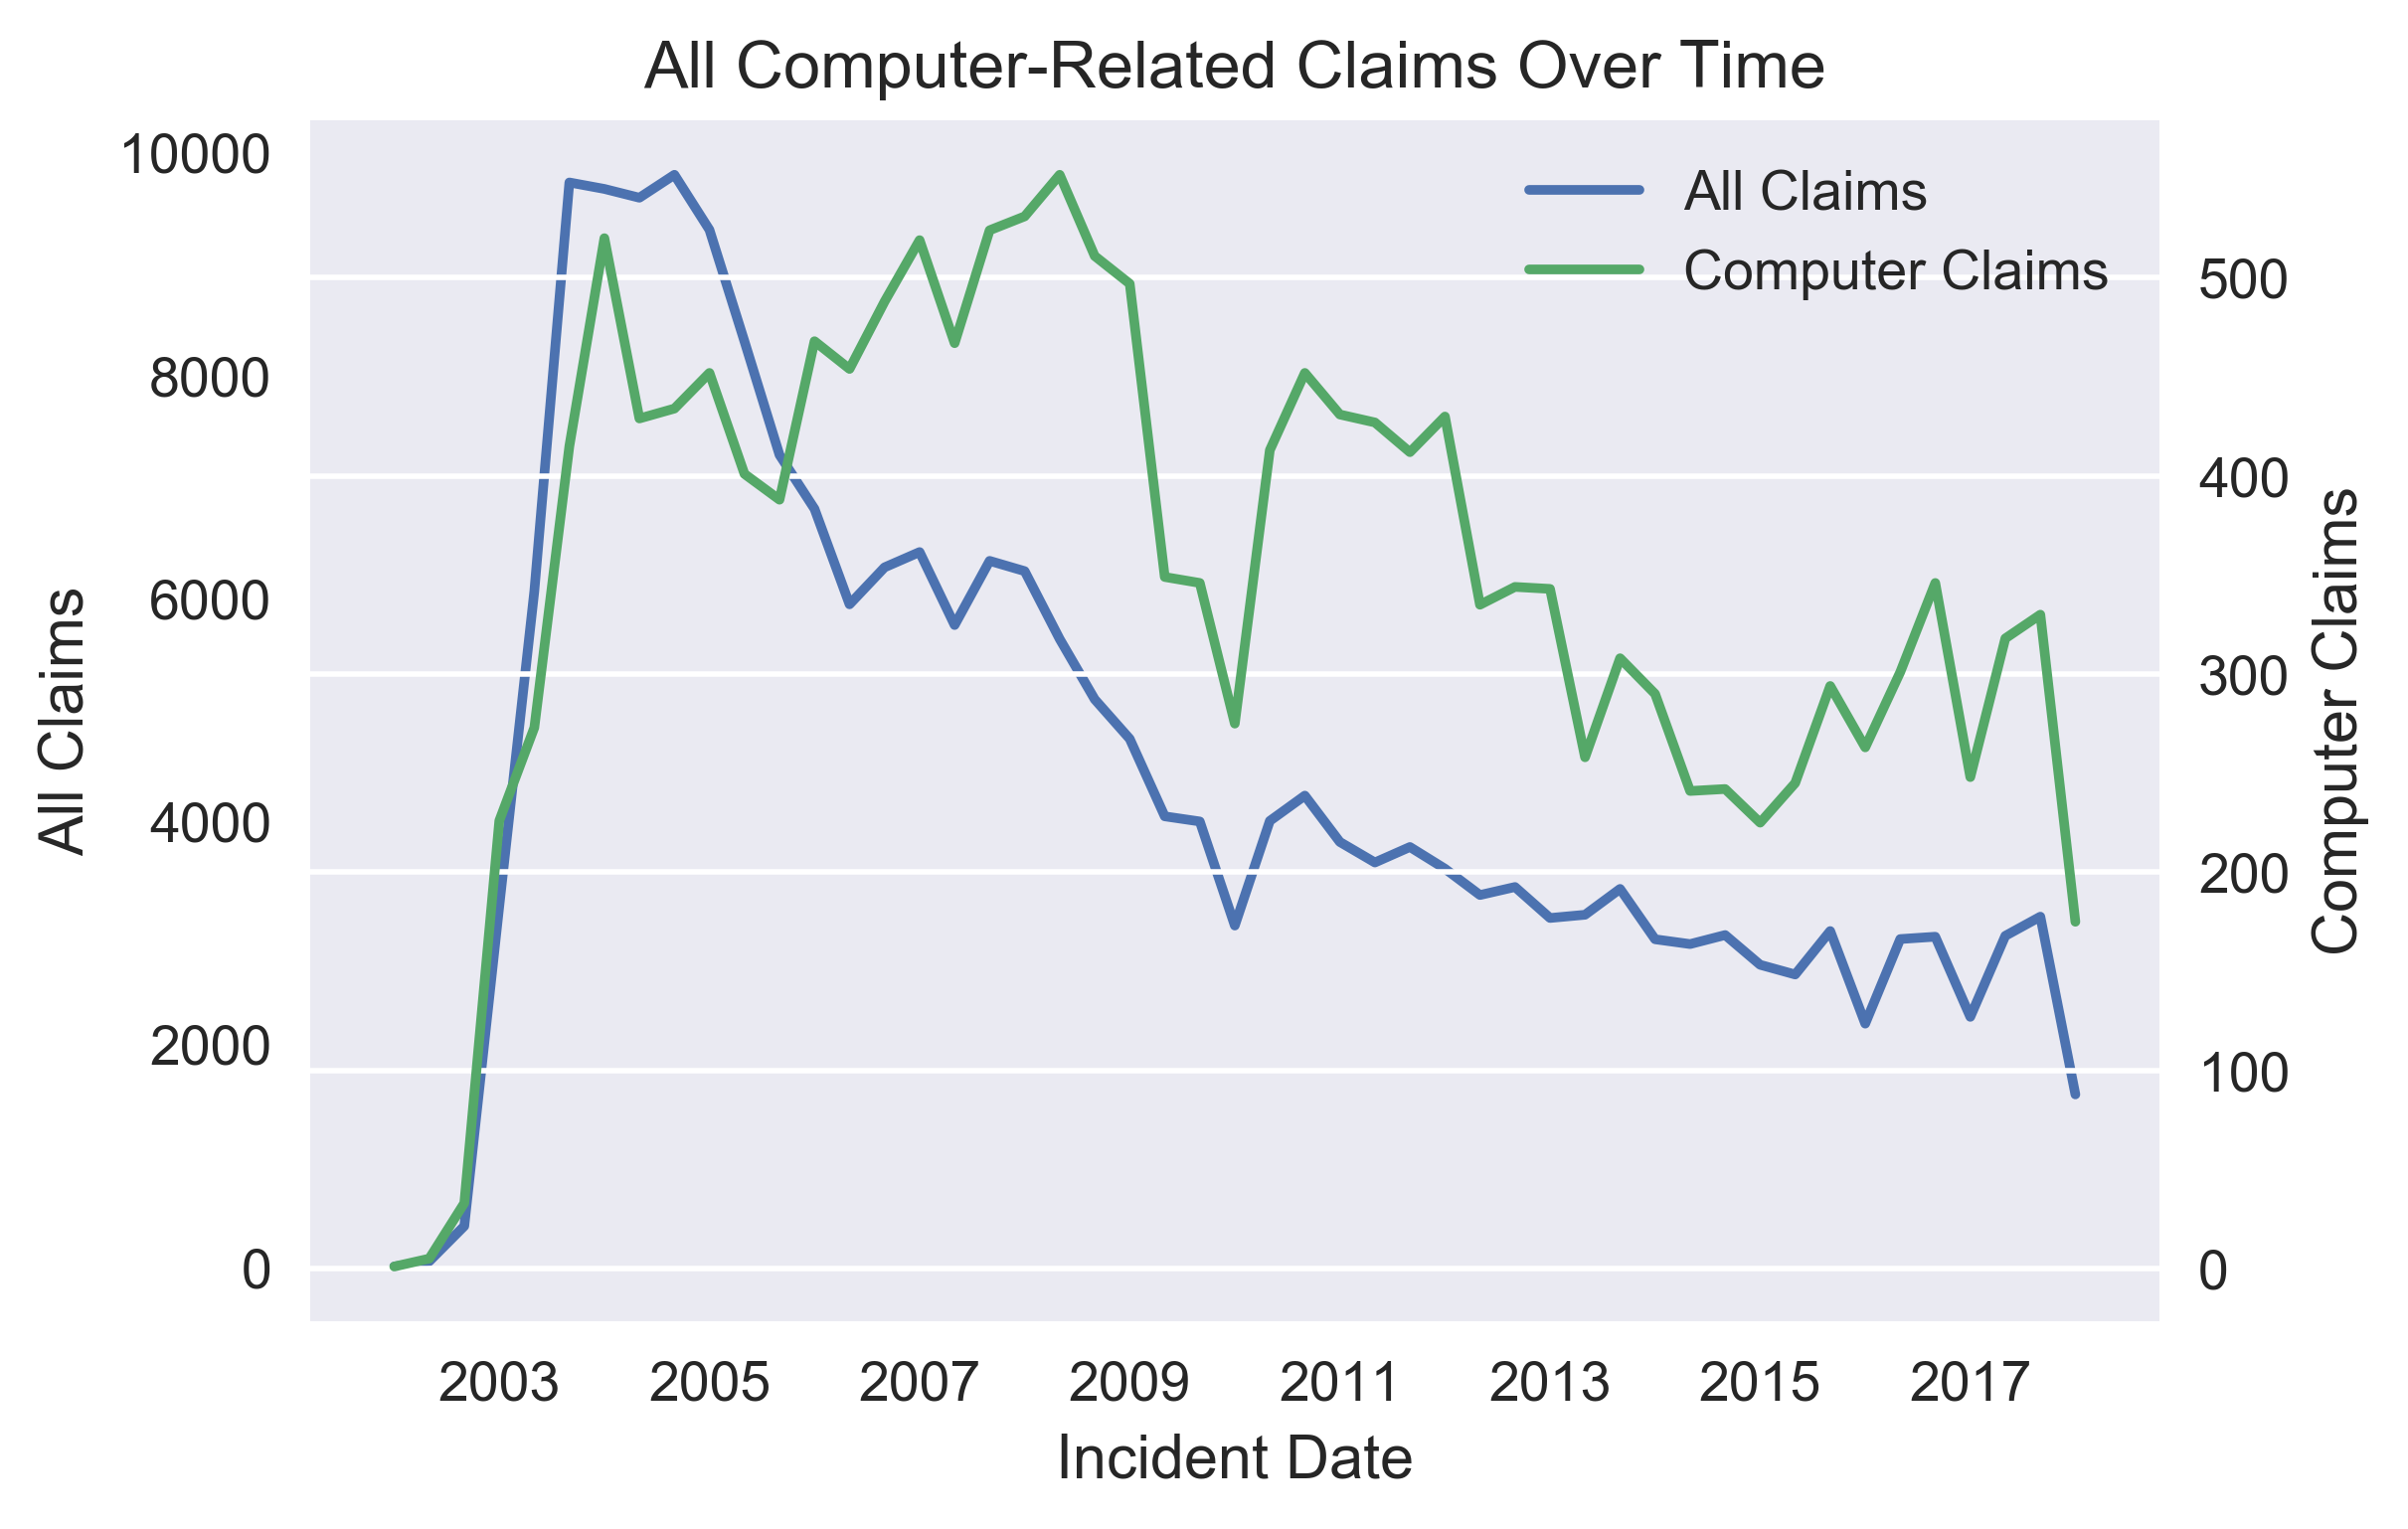
\includegraphics[keepaspectratio, width = \textwidth, height = \textheight]{../plots/computers}
\end{frame}

\begin{frame}
	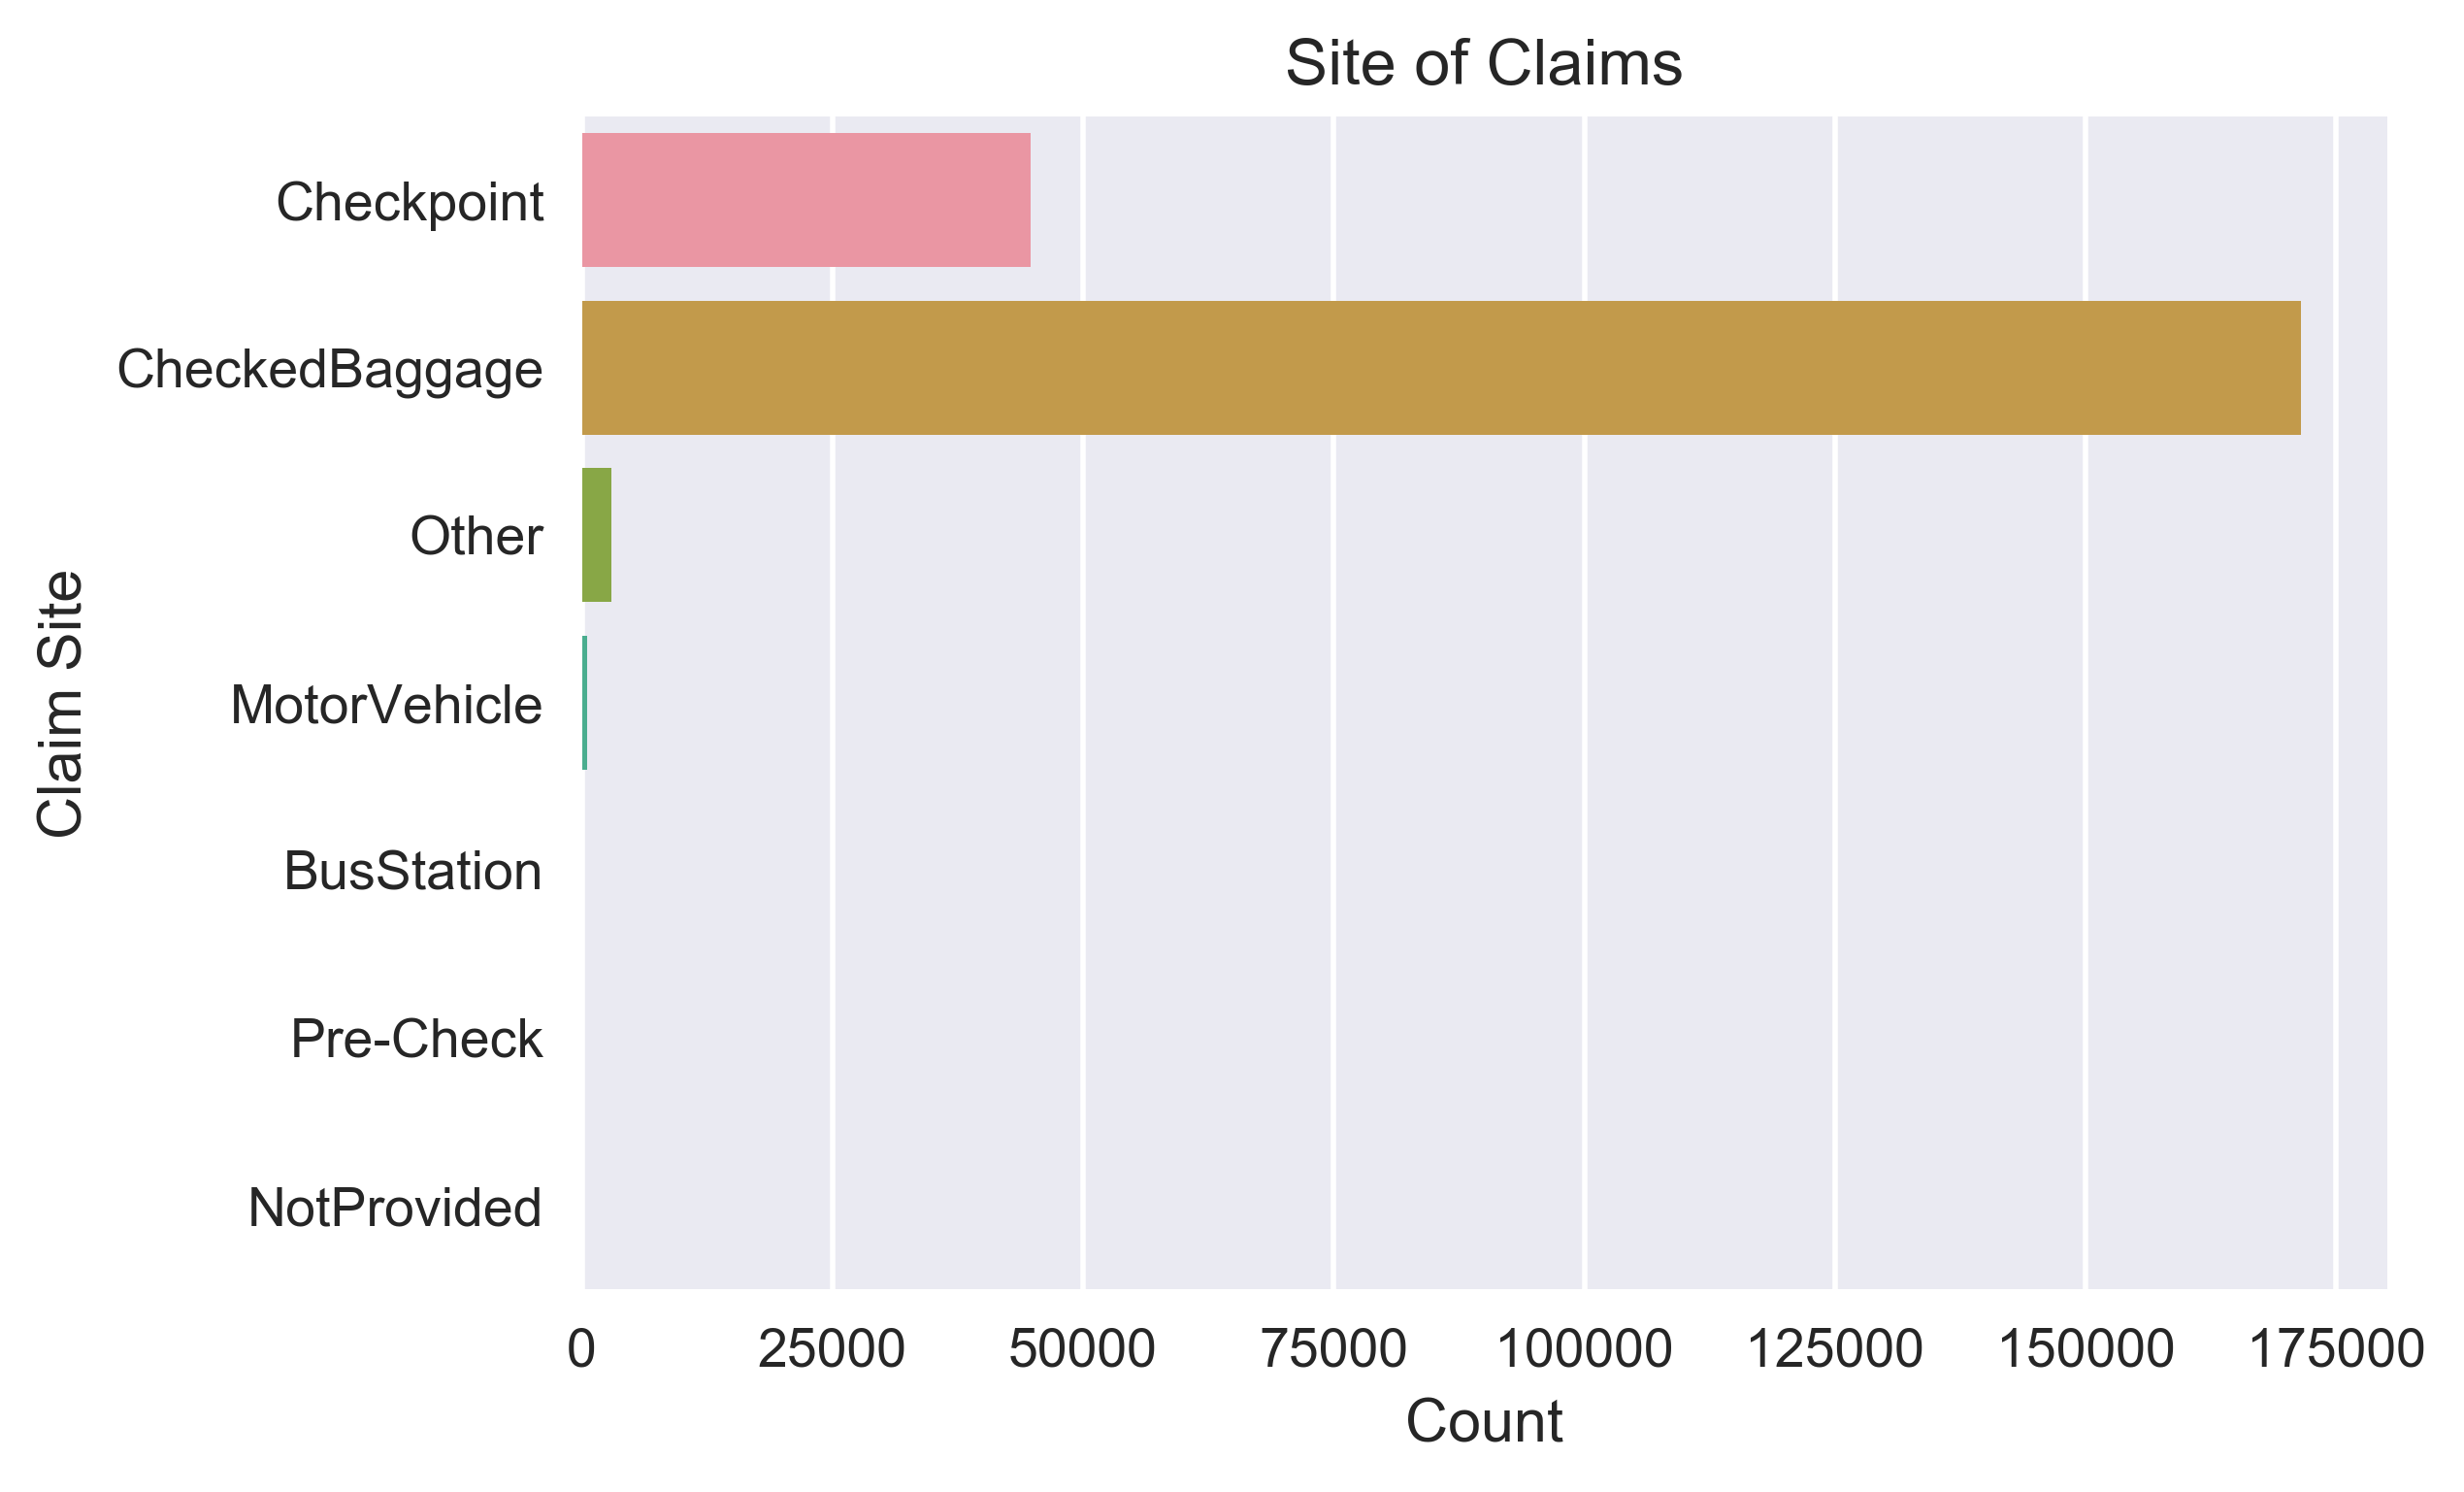
\includegraphics[keepaspectratio, width = \textwidth, height = \textheight]{../plots/sites}
\end{frame}

\begin{frame}
	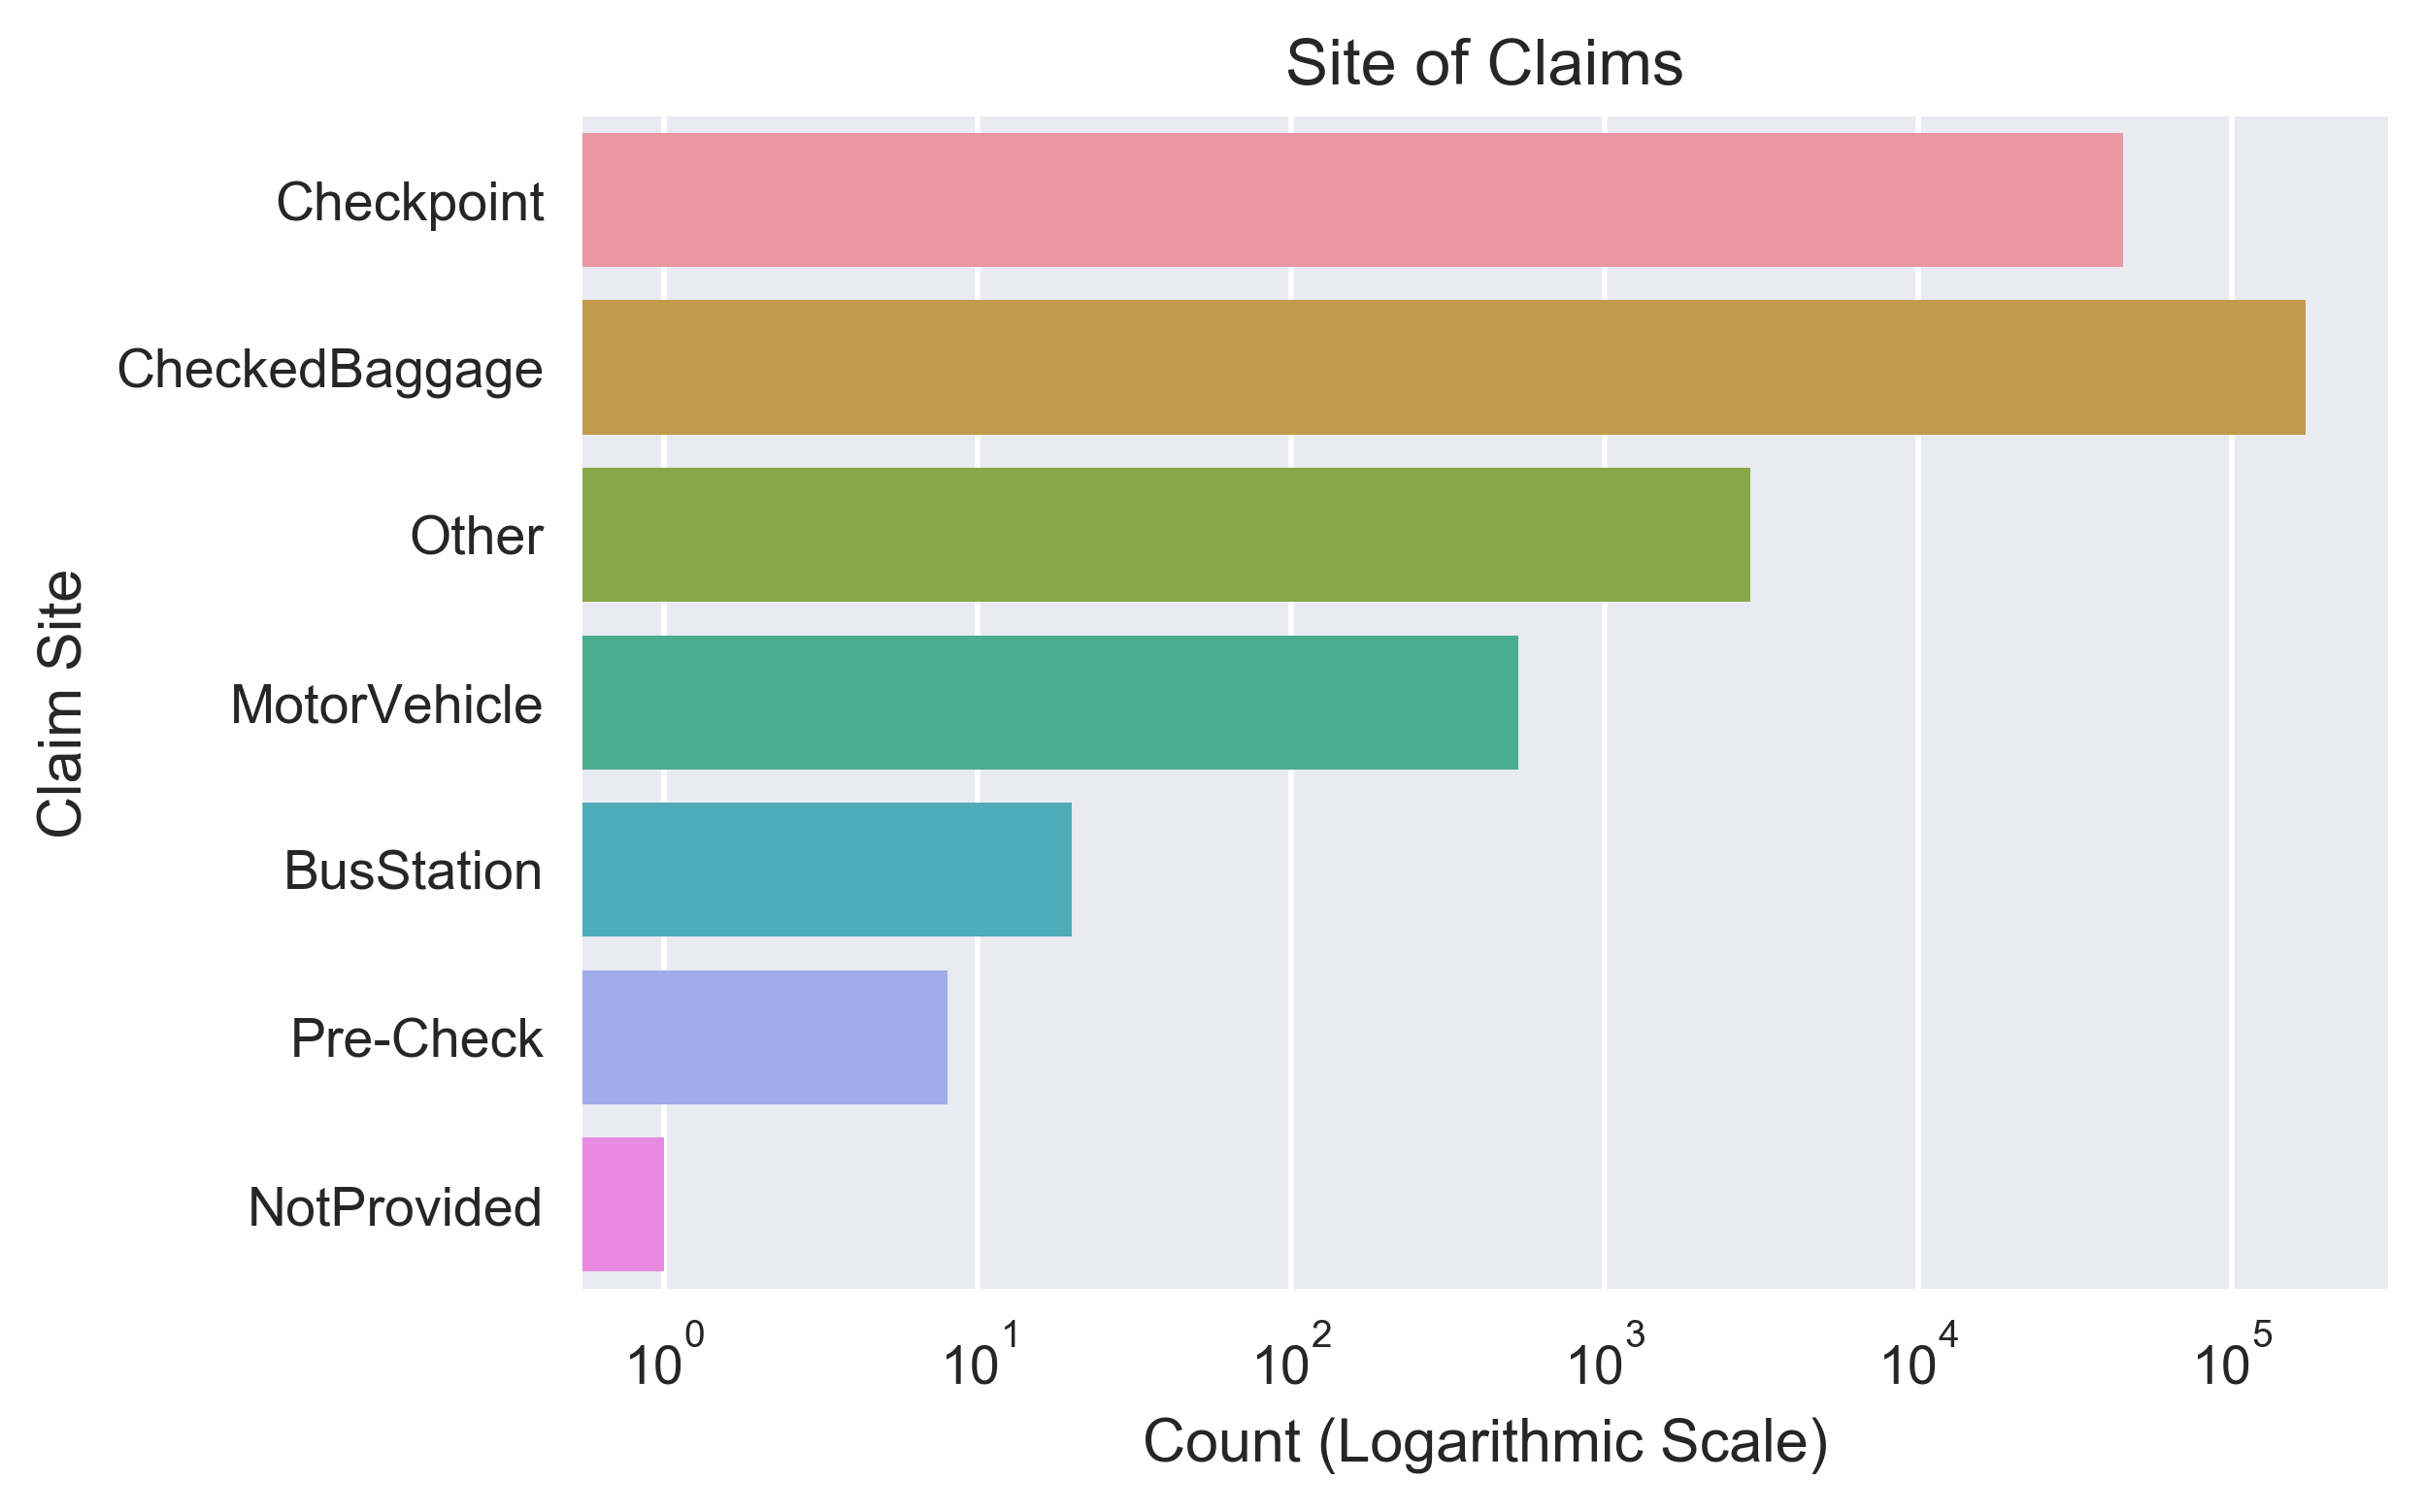
\includegraphics[keepaspectratio, width = \textwidth, height = \textheight]{../plots/log_sites}
\end{frame}

\end{document}
